\documentclass[11pt]{article}

% ============================================================
% PAQUETES
% ============================================================
\usepackage[utf8]{inputenc}
\usepackage[T1]{fontenc}
\usepackage[spanish,es-noindentfirst]{babel}
\usepackage{lmodern}
\usepackage[a4paper,margin=2.4cm,headheight=14pt]{geometry}
\usepackage{amsmath,amssymb}
\usepackage{graphicx}
\usepackage{subcaption}
\usepackage{booktabs}
\usepackage{array}
\usepackage{caption}
\usepackage[table]{xcolor}
\usepackage{enumitem}
\usepackage{fancyhdr}
\usepackage{titlesec}
\usepackage{abstract}
\usepackage[colorlinks=true,linkcolor=blue!50!black,citecolor=blue!50!black,urlcolor=blue!50!black]{hyperref}
\usepackage[capitalise,spanish]{cleveref}

% ---------- Tipografía de títulos ----------
\titleformat{\section}{\normalfont\Large\bfseries}{\thesection.}{0.6em}{}
\titleformat{\subsection}{\normalfont\large\bfseries}{\thesubsection.}{0.6em}{}
\titleformat{\subsubsection}{\normalfont\normalsize\bfseries\itshape}{\thesubsubsection.}{0.5em}{}
\titlespacing*{\section}{0pt}{1.4em}{0.7em}
\titlespacing*{\subsection}{0pt}{1.1em}{0.5em}

% ---------- Nombres en español (babel fija \captionsspanish en \begin{document}, ----------
% ---------- así que los ajustes deben engancharse ahí, no con \renewcommand directo) ----
\addto\captionsspanish{%
  \renewcommand{\figurename}{Figura}%
  \renewcommand{\tablename}{Tabla}%
  \renewcommand{\refname}{Referencias}%
  \renewcommand{\abstractname}{Resumen}%
}

% ---------- Encabezados ----------
\pagestyle{fancy}
\fancyhf{}
\renewcommand{\headrulewidth}{0.4pt}
\fancyhead[L]{\small\itshape Ortiz Carreño y Haro Mendoza}
\fancyhead[R]{\small\itshape Rendezvous modular para tripletes quirúrgicos}
\fancyfoot[C]{\small\thepage}

% ---------- Captions ----------
\captionsetup{font=small,labelfont=bf,justification=justified,margin=0.5cm}
\captionsetup[subfigure]{labelformat=simple,labelsep=colon}
\renewcommand{\thesubfigure}{\alph{subfigure}}

% ---------- Enlaces de figura/tabla con nombre correcto ----------
\crefname{figure}{Figura}{Figuras}
\Crefname{figure}{Figura}{Figuras}
\crefname{table}{Tabla}{Tablas}
\Crefname{table}{Tabla}{Tablas}
\crefname{section}{Sección}{Secciones}
\Crefname{section}{Sección}{Secciones}
\crefname{equation}{Ecuación}{Ecuaciones}

\setlength{\parskip}{0.25em}

\title{\LARGE\bfseries Implementación Modular y Adaptación de la Arquitectura Rendezvous para el Reconocimiento de Tripletes Quirúrgicos en Colecistectomía Laparoscópica bajo Restricciones de Hardware}

\author{
Fabián Ortiz Carreño \\
{\small Ingeniería Mecatrónica, Facultad de Ingeniería} \\
{\small Universidad Nacional Autónoma de México} \\
{\small\texttt{ortizcarreno.fabian@ejemplo.com}}
\and
Daniel Haro Mendoza \\
{\small Asesor, Facultad de Ingeniería} \\
{\small Universidad Nacional Autónoma de México}
}

\date{Ciudad Universitaria, México. Semestre 2026-2}

\begin{document}

\maketitle
\thispagestyle{fancy}

\begin{abstract}
El reconocimiento automático de tripletes quirúrgicos ⟨instrumento, verbo, órgano⟩ en video laparoscópico es una tarea central para la cirugía asistida por inteligencia artificial, pero su entrenamiento extremo a extremo con arquitecturas como Rendezvous (RDV) exige recursos de cómputo —memoria VRAM y clústeres multi-GPU— que están fuera del alcance de la mayoría de los entornos académicos. Este trabajo presenta una reimplementación modular de la arquitectura RDV, diseñada explícitamente para operar en una única GPU de consumo de 3~GB de VRAM, y evaluada sobre el conjunto de datos CholecT50. Se muestra que el entrenamiento monolítico con \emph{backbone} congelado sufre de \textbf{competencia de gradientes}: los gradientes de alta magnitud asociados a los bordes metálicos de los instrumentos dominan la retropropagación y bloquean el aprendizaje anatómico, estancando la precisión promedio de órganos (AP) en 19.52\,\%. Como alternativa se propone una estrategia de \textbf{especialistas aislados} —instrumentos, verbos y órganos entrenados de forma independiente— seguida de una \textbf{fase de fusión} con ajuste fino extremo a extremo a tasa de aprendizaje restrictiva, y de una \textbf{integración espaciotemporal} mediante una Red Convolucional Temporal (TCN) que opera sobre características extraídas fuera de línea. La especialización aislada eleva el AP anatómico a 27.35\,\% (instrumentos: 86.42\,\%; verbos: 54.02\,\%), y la variante espaciotemporal final (SpatioTemporalRDV) alcanza mAP\textsubscript{I}\,=\,77.56\,\%, mAP\textsubscript{V}\,=\,53.59\,\%, mAP\textsubscript{T}\,=\,38.45\,\% y mAP\textsubscript{IVT}\,=\,13.38\,\% sobre el Fold~1 de CholecT50 —un incremento de 6.5$\times$ en mAP\textsubscript{IVT} respecto a la variante estática local (2.06\,\%)—, evaluada íntegramente en un equipo portátil con GPU NVIDIA GTX~1050. Los resultados, obtenidos en un solo \emph{fold} y sin \emph{ablation study} formal, se interpretan como evidencia empírica a favor de la hipótesis de aislamiento de gradientes y como una vía metodológica viable para investigar arquitecturas de reconocimiento quirúrgico fuera de infraestructura multi-GPU, sin pretender una superación del estado del arte.

\smallskip
\noindent\textbf{Palabras clave:} reconocimiento de tripletes quirúrgicos; arquitectura Rendezvous; cirugía laparoscópica; CholecT50; aprendizaje profundo con restricciones de hardware; redes convolucionales temporales; competencia de gradientes.
\end{abstract}

\section{Introducción}
\label{sec:intro}

\subsection{Contexto}
\label{sec:contexto}

La cirugía laparoscópica moderna, y en particular procedimientos como la colecistectomía (extracción de la vesícula biliar), depende de una cámara endoscópica introducida en el abdomen del paciente. Esta cámara genera un volumen masivo de datos visuales en tiempo real cuyo análisis manual resulta inabarcable \cite{dergachyova2016}. Comprender automáticamente lo que ocurre en estos videos se considera uno de los problemas centrales de la inteligencia artificial aplicada a la medicina computacional.

Una máquina capaz de interpretar el flujo quirúrgico no solo permitiría evaluar de forma objetiva las habilidades de cirujanos novatos, sino que sentaría las bases computacionales para quirófanos autónomos o semiautónomos del futuro \cite{twinanda2017}. Alcanzar ese nivel de comprensión exige que la inteligencia artificial no se limite a la detección de objetos aislados: debe decodificar el \emph{triplete quirúrgico}, es decir, la relación semántica exacta y simultánea entre un instrumento, la acción (verbo) que realiza y el órgano sobre el que actúa —por ejemplo, ⟨\emph{Grasper}, \emph{Retract}, \emph{Gallbladder}⟩— \cite{nwoye2022rendezvous}.

\subsection{Problemática}
\label{sec:problematica}

El desarrollo de algoritmos capaces de extraer esta información semántica enfrenta obstáculos físicos y computacionales sumamente restrictivos:

\begin{enumerate}[label=\arabic*)]
    \item \textbf{El desafío del ``mar rosa'' (similitud anatómica).} A diferencia de la visión por computadora en entornos estructurados, el intraabdomen es un escenario de alta ambigüedad visual. Los tejidos blandos —hígado, vesícula, tejido adiposo, peritoneo— exhiben texturas, colores y propiedades reflectantes casi idénticas, lo que genera alta variabilidad intra-clase y baja variabilidad inter-clase.
    \item \textbf{Entorno visual adverso.} Las imágenes endoscópicas están constantemente degradadas por artefactos dinámicos: humo generado por el electrobisturí, reflejos especulares causados por la humedad de los tejidos, cambios bruscos en la iluminación y oclusión de la anatomía por los instrumentos metálicos.
    \item \textbf{Restricciones computacionales.} Modelar la relación simultánea de 100 clases posibles de tripletes exige arquitecturas de aprendizaje profundo de alto costo paramétrico. El entrenamiento extremo a extremo colapsa rápidamente la memoria VRAM de estaciones de trabajo estándar, imponiendo la necesidad de reestructurar la ingeniería del entrenamiento computacional.
\end{enumerate}

Este último punto es el eje del presente trabajo: mientras que el estado del arte en reconocimiento de tripletes quirúrgicos se ha desarrollado casi exclusivamente sobre infraestructura de clúster multi-GPU, un volumen considerable de investigación académica —particularmente en instituciones con recursos computacionales limitados— no tiene acceso a dicha infraestructura. Cerrar esa brecha metodológica, sin renunciar a la fidelidad del mecanismo de atención de dos niveles que caracteriza al estado del arte, es la motivación central de este artículo.

\subsection{Contribuciones}
\label{sec:contribuciones}

Este trabajo presenta y evalúa empíricamente una reingeniería del entrenamiento de la arquitectura Rendezvous (RDV) orientada a hardware de consumo de un solo GPU de 3~GB de VRAM. Las contribuciones específicas son:

\begin{itemize}[leftmargin=1.4em]
    \item Un diagnóstico cuantitativo del fenómeno de \textbf{competencia de gradientes} en el entrenamiento monolítico con \emph{backbone} congelado, sustentado en la evolución del AP por dominio semántico y en matrices de confusión por época (\cref{sec:resultados-monolitico}).
    \item Una estrategia de \textbf{especialistas aislados} —instrumentos, verbos y órganos— que descompone el entrenamiento extremo a extremo en subproblemas desacoplados, seguida de una \textbf{fase de fusión} con ajuste fino de tasa de aprendizaje restrictiva (\cref{sec:metodologia}).
    \item Una arquitectura de \textbf{extracción de características fuera de línea} acoplada a una Red Convolucional Temporal (TCN), que introduce contexto espaciotemporal sin exceder la memoria disponible (\cref{sec:tcn}).
    \item Un diagnóstico matemático y la corrección de dos deficiencias estructurales —truncamiento de gradientes negativos por ReLU y logits de baja magnitud— que bloqueaban la convergencia de la fase de fusión (\cref{sec:diagnostico-matematico}).
    \item Una evaluación empírica sobre el Fold~1 de CholecT50, con comparación explícita y metodológicamente acotada frente al estado del arte (\cref{sec:comparativa}), junto con una discusión transparente de las limitaciones de protocolo (\cref{sec:limitaciones}).
\end{itemize}

El resto del artículo se organiza como sigue. La \cref{sec:fundamentos} describe la arquitectura Rendezvous original y su desempeño de referencia. La \cref{sec:metodologia} detalla la metodología propuesta. La \cref{sec:protocolo} describe el protocolo experimental. La \cref{sec:resultados} presenta los resultados a lo largo de los tres horizontes de desarrollo. La \cref{sec:discusion} discute su significado, alcance y limitaciones, y las \cref{sec:conclusiones,sec:trabajo-futuro} cierran con las conclusiones y el trabajo futuro.

\section{Fundamentos: la arquitectura Rendezvous}
\label{sec:fundamentos}

El modelo Rendezvous (RDV) \cite{nwoye2022rendezvous} reconoce tripletes directamente desde el video quirúrgico aprovechando mecanismos de atención en dos niveles distintos. Su flujo de procesamiento se compone de las siguientes etapas:

\begin{itemize}[leftmargin=1.4em]
    \item \textbf{Extracción de características (\emph{backbone}).} La imagen de entrada es procesada por una ResNet-18 que extrae características de alto y bajo nivel.
    \item \textbf{Codificador (atención espacial).} Una capa de Localización Débilmente Supervisada (WSL) ubica los instrumentos; el Mecanismo de Atención Guiado por Activación de Clases (CAGAM) enfoca el reconocimiento de verbos y órganos usando las activaciones de los instrumentos; y una capa cuello de botella (\emph{bottleneck}) recopila características sin filtrar.
    \item \textbf{Decodificador (atención semántica).} El módulo de Múltiples Cabezales de Atención Mixta (MHMA), inspirado en redes Transformer, emplea auto-atención y atención cruzada para capturar las relaciones entre instrumentos, verbos y órganos.
\end{itemize}

En su evaluación sobre el conjunto de datos CholecT50 —50 videos endoscópicos con anotaciones para 100 clases de tripletes—, el modelo RDV estableció métricas de referencia mundiales: AP de 92.0\,\% para instrumentos, 60.7\,\% para verbos y 38.3\,\% para órganos, con un AP de triplete completo (mAP\textsubscript{IVT}) del 29.9\,\% \cite{nwoye2022rendezvous}. Estos resultados se obtuvieron mediante validación cruzada de 5 \emph{folds} sobre CholecT50 utilizando infraestructura de clúster multi-GPU, un punto que resulta central para interpretar correctamente las comparaciones de la \cref{sec:comparativa}.

\section{Metodología}
\label{sec:metodologia}

\subsection{Reducción del Rendezvous original para hardware de recursos limitados}
\label{sec:reduccion}

El entrenamiento original de la arquitectura RDV es de naturaleza extremo a extremo (\emph{end-to-end}): requiere calcular, almacenar y actualizar los gradientes de millones de parámetros simultáneamente en cada iteración, desde la ResNet-18 hasta las capas del decodificador MHMA. Este enfoque monolítico exige una cantidad masiva de memoria VRAM, limitando su ejecución viable a clústeres de supercómputo o servidores de alto rendimiento.

Para viabilizar este proyecto en una estación de trabajo móvil convencional —Lenovo IdeaPad Gaming con procesador Intel Core i5-9300H a 2.40~GHz, 16.0~GB de RAM DDR4 a 2400~MHz, GPU NVIDIA GeForce GTX~1050 (3~GB VRAM) y SSD Kingston SA400S37480G de 447~GB—, fue necesario aplicar estrategias de reducción de carga computacional. El primer intento —documentado en el \emph{script} base \texttt{run.py}— se centró en el congelamiento de pesos (\emph{freezing}): se bloqueó la retropropagación en todas las capas de la ResNet-18, transformándola en un extractor de características estático. Esto liberó suficiente memoria VRAM para intentar entrenar las ramas de instrumentos, verbos y órganos de forma simultánea.

Sin embargo, este enfoque monolítico congelado presentó una deficiencia matemática crítica: la \textbf{competencia de gradientes}. Al optimizar los tres componentes en un solo paso hacia atrás mediante una función de pérdida combinada con pesos iguales para cada rama, los errores competían entre sí durante la retropropagación. Los gradientes asociados a los bordes metálicos de alta frecuencia espacial de los instrumentos poseían magnitudes dominantes y aplastaban los gradientes de menor norma requeridos para aprender las texturas anatómicas. Esto estancó el mAP\textsubscript{T} en un deficiente 19.52\,\%. Esta limitación —tanto de hardware como matemática— fue el catalizador que obligó a diseñar la metodología de especialistas aislados descrita a continuación.

\begin{figure}[htbp]
    \centering
    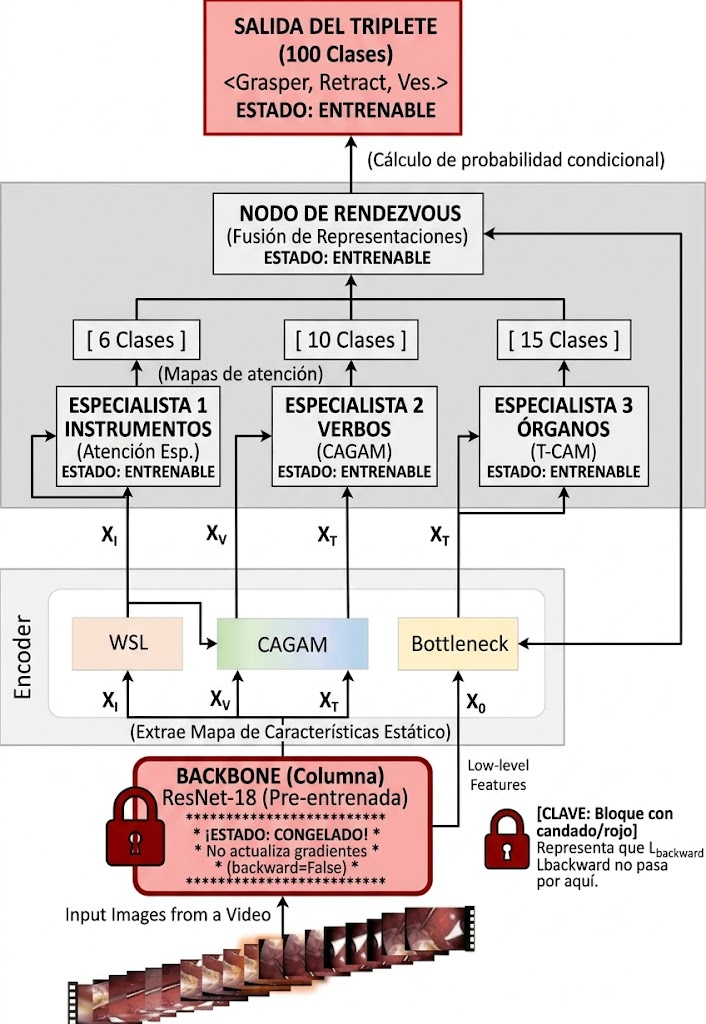
\includegraphics[width=0.55\linewidth]{figures/fig01_freezing_architecture.png}
    \caption{Adaptación de la arquitectura Rendezvous mediante congelamiento de pesos (\emph{freezing}). El símbolo de candado indica que la retropropagación no actualiza el \emph{backbone}. Adaptado de \cite{nwoye2023cholectriplet}.}
    \label{fig:freezing}
\end{figure}

\subsection{Metodología de especialistas aislados}
\label{sec:especialistas}

Al diagnosticar la competencia de gradientes, se tomó la decisión arquitectónica de desvincular la red en \textbf{tres módulos independientes}, denominados ``especialistas''. En lugar de forzar a una sola red a optimizar tres dominios semánticos dispares con una única función de pérdida, cada especialista recibe su propio entorno de optimización, tasa de aprendizaje y tiempo de maduración.

El flujo de trabajo de la especialización aislada comprende las siguientes etapas:

\begin{enumerate}[leftmargin=1.6em]
    \item \textbf{Especialista 1 — Instrumentos (guía espacial).} Se descongeló la ResNet-18 exclusivamente para esta tarea. Al entrenar la red sobre las 6 clases de herramientas metálicas, el modelo aprendió a generar mapas de atención precisos. Esta etapa es el cimiento de la arquitectura, pues los instrumentos dictan hacia dónde deben dirigir su análisis los módulos posteriores.
    \item \textbf{Especialista 2 — Órganos (T-CAM).} Con la base de instrumentos consolidada, se entrenó la rama anatómica sobre 15 clases. Al aislar este entrenamiento, el optimizador concentró toda la retropropagación en resolver el problema del ``mar rosa'', aprendiendo a diferenciar texturas de tejidos blandos sin la interferencia de los demás dominios.
    \item \textbf{Especialista 3 — Verbos (CAGAM).} Se aisló el módulo de acciones quirúrgicas sobre 10 clases. La red utilizó la información espacial heredada de los instrumentos —mediante el mecanismo CAGAM— para deducir qué acción se ejecutaba en cada coordenada.
\end{enumerate}

\begin{figure}[htbp]
    \centering
    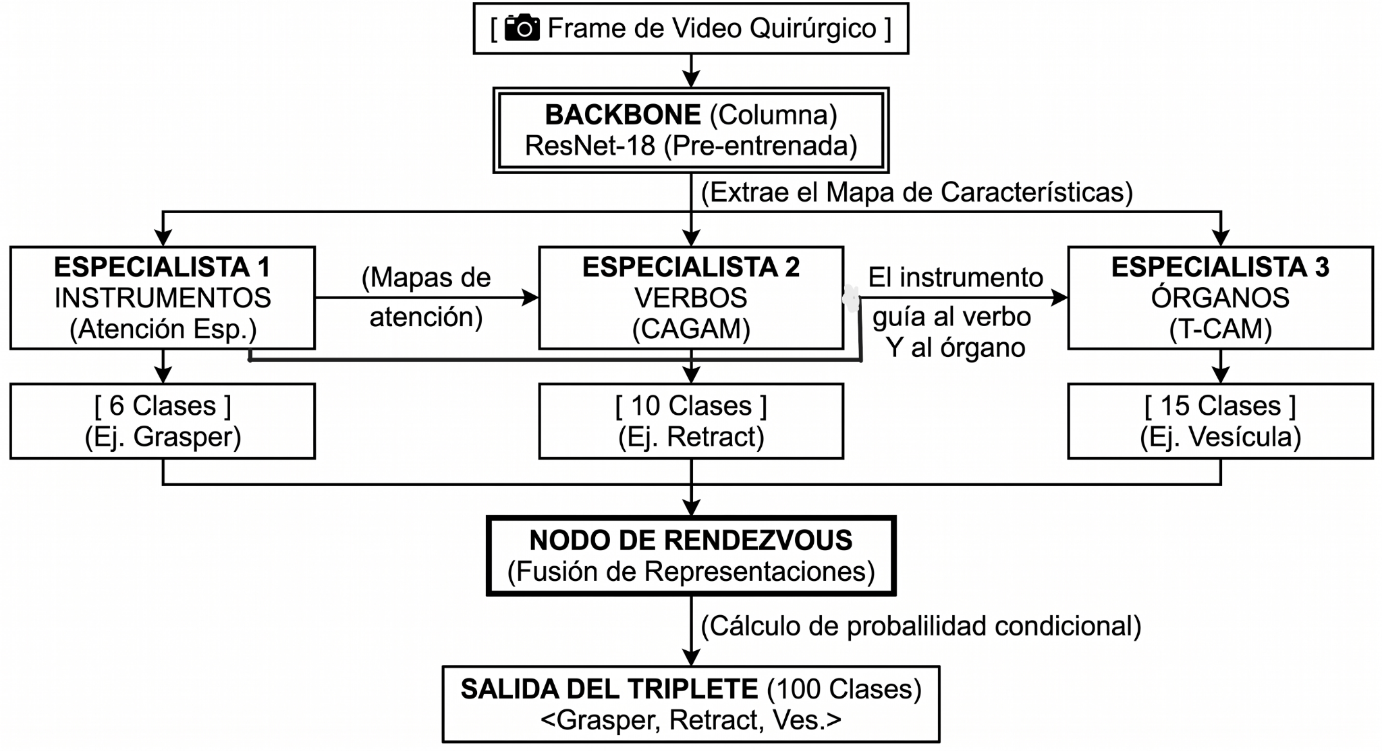
\includegraphics[width=\linewidth]{figures/fig02_specialists_architecture.png}
    \caption{Arquitectura interna del modelo RDV estructurada por especialistas. El módulo de instrumentos actúa como guía direccional, inyectando sus mapas de atención tanto al módulo CAGAM (verbos) como al T-CAM (órganos). El Nodo de Rendezvous infiere la probabilidad condicional del triplete completo. Adaptado de \cite{nwoye2023cholectriplet}.}
    \label{fig:especialistas}
\end{figure}

\subsection{Fase de fusión (ajuste fino extremo a extremo)}
\label{sec:fusion}

Una vez que los tres especialistas alcanzaron su rendimiento máximo de forma aislada, se procedió a la \textbf{fase de fusión}. Los pesos pre-entrenados de cada módulo se inyectaron en una arquitectura RDV unificada, y se liberó la propagación de gradientes completa (\emph{end-to-end fine-tuning}) con una tasa de aprendizaje restrictiva del orden de $8 \times 10^{-5}$. Esta restricción permite que los módulos desarrollen co-adaptación —dejando de ser expertos individuales para convertirse en un equipo capaz de inferir el triplete completo— sin destruir las representaciones previas.

\subsection{Integración espaciotemporal (TCN) y optimización de hardware}
\label{sec:tcn}

Durante el análisis de resultados del especialista de verbos, se corroboró una limitación intrínseca del análisis estático por fotograma. Acciones quirúrgicas complejas como ``Retraer'' (\emph{Retract}) o ``Diseccionar'' (\emph{Dissect}) son inherentemente eventos espaciotemporales: su naturaleza semántica reside en la cinemática del movimiento a lo largo del tiempo, no en un encuadre aislado.

Para dotar al modelo de esta memoria secuencial, se integró una Red Convolucional Temporal (\emph{Temporal Convolutional Network}, TCN). A diferencia de las redes recurrentes (LSTM), las TCN emplean convoluciones dilatadas que procesan secuencias en paralelo, evitando el problema de desvanecimiento del gradiente propio del entrenamiento de redes recurrentes profundas. No obstante, esta ventaja tiene un costo acotado: las TCN poseen un \textbf{campo receptivo fijo}, determinado por la profundidad de la red y los factores de dilatación, lo que puede limitar su desempeño ante dependencias temporales de rango variable más allá de dicho campo. El \emph{pipeline} de extracción de características procesa los videos de CholecT50 a una tasa muestreada de 1 fotograma por segundo (1~fps), consistente con el protocolo de anotación del conjunto de datos; esta tasa es la que determina que el campo receptivo de 17 fotogramas de la TCN (\cref{tab:tcn}) equivalga a una ventana temporal de aproximadamente 17 segundos.

\begin{table}[htbp]
    \centering
    \caption{Especificación arquitectónica de la Red Convolucional Temporal (TCN) implementada.}
    \label{tab:tcn}
    \small
    \begin{tabular}{@{}ll@{}}
        \toprule
        \textbf{Parámetro} & \textbf{Valor} \\
        \midrule
        Número de bloques & 4 (\texttt{num\_channels}=[256,256,256]) \\
        Tamaño de kernel & 3 \\
        Dilataciones por bloque & 1, 2, 4, 8 (exponencial) \\
        Campo receptivo efectivo & 17 fotogramas ($\approx$17\,s a 1\,fps) \\
        Tipo de \emph{padding} & Bidireccional (no causal) \\
        Normalización & BatchNorm1d por bloque \\
        Dropout & 0.3 \\
        Dimensión de entrada & [Batch, 512, $T$] \\
        Cabezales de salida & 4 capas Conv1d 1$\times$1: 6, 10, 15 y 100 clases \\
        \bottomrule
    \end{tabular}
\end{table}

El diseño bidireccional (no causal) es deliberado: dado que CholecT50 consiste en videos pregrabados, el sistema puede explotar contexto temporal tanto pasado como futuro para suavizar el \emph{flickering} de predicciones fotograma a fotograma, sin la restricción de inferencia en tiempo real.

Acoplar la TCN de forma simultánea con el \emph{backbone} ResNet-18 excedía drásticamente la memoria VRAM disponible (3~GB). Para solucionar este cuello de botella, se diseñó una arquitectura de \textbf{extracción fuera de línea} (\emph{offline}) con el siguiente \emph{pipeline}:

\begin{enumerate}[leftmargin=1.6em]
    \item \textbf{Extracción espacial estática.} Utilizando los especialistas aislados como extractores de características con pesos congelados, se iteró todo el conjunto de datos para pre-calcular los Mapas de Activación de Clases (CAMs 2D) y los vectores de 512 dimensiones por fotograma, almacenándolos en disco.
    \item \textbf{Suavizado temporal.} Los vectores espaciales de cada video completo se procesaron a través de la TCN (pre-entrenada y congelada) para generar logits de probabilidad suavizados en el eje del tiempo.
    \item \textbf{Carga en RAM y fusión eficiente.} El conjunto de CAMs y vectores temporales se cargó íntegramente en los 16~GB de RAM del sistema. Esta estrategia eliminó el cuello de botella de latencia por E/S de disco, reduciendo el tiempo de optimización de múltiples horas a un promedio de 21 segundos por época en la estación de trabajo descrita.
\end{enumerate}

Cabe precisar una implicación metodológica importante de esta estrategia: dado que los vectores de características se pre-calculan y congelan antes del entrenamiento del módulo de fusión, el \emph{backbone} no puede co-adaptarse durante dicho entrenamiento. El ajuste fino resultante no es, en sentido estricto, completamente extremo a extremo, sino una optimización de las capas superiores sobre representaciones fijas. Esta restricción se impone por las limitaciones de hardware y constituye un compromiso de diseño explícito, retomado en la \cref{sec:limitaciones}.

\begin{figure}[htbp]
    \centering
    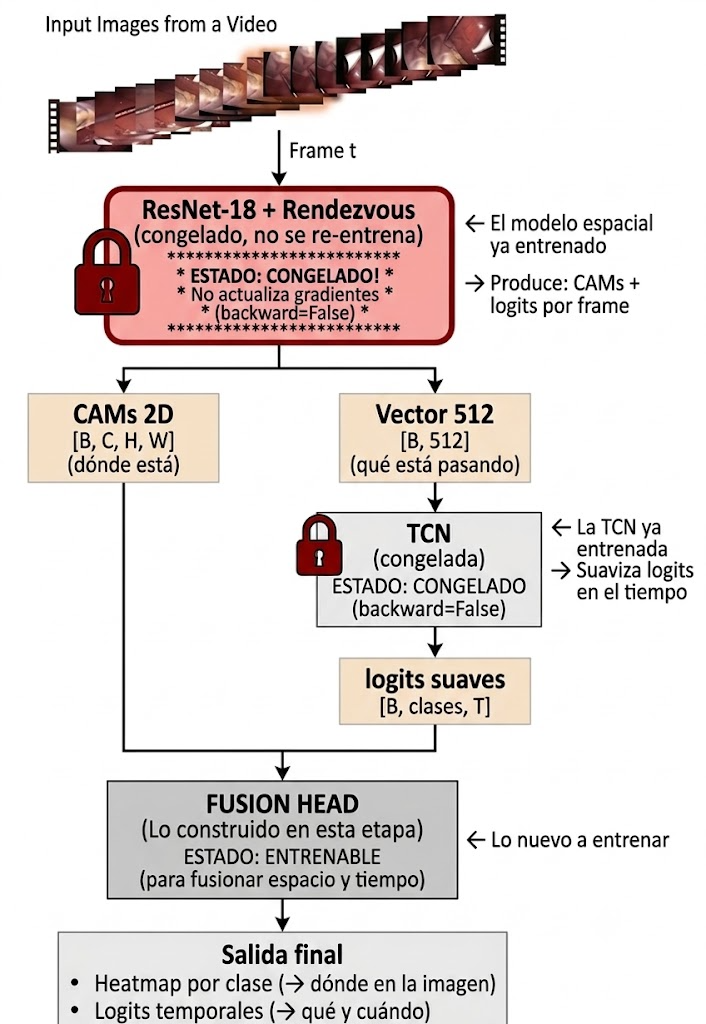
\includegraphics[width=0.55\linewidth]{figures/fig03_spatiotemporal_pipeline.png}
    \caption{Flujo de datos de la arquitectura espaciotemporal implementada. El \emph{pipeline} extrae los mapas de atención (CAMs) y las características profundas de forma aislada, utilizando la TCN para condicionar temporalmente el módulo de fusión final entrenable.}
    \label{fig:pipeline}
\end{figure}

\section{Protocolo experimental}
\label{sec:protocolo}

\subsection{Conjunto de datos y partición}
\label{sec:particion}

El entrenamiento y la evaluación se realizaron sobre el conjunto de datos \textbf{CholecT50}, compuesto por 50 videos de colecistectomía laparoscópica con anotaciones para 100 clases de tripletes. Para los especialistas aislados y el modelo de fusión se siguió el esquema de validación cruzada de 5 \emph{folds} definido en el \emph{benchmark} CholecTriplet2021 \cite{nwoye2023cholectriplet}, con separación estricta por paciente.

La evaluación cuantitativa reportada en este trabajo se realizó exclusivamente sobre los \textbf{9 videos del Fold~1} de dicho protocolo: VID002, VID006, VID014, VID023, VID025, VID050, VID051, VID066 y VID079. Esta selección es consistente entre todas las variantes comparadas (RDV Local y SpatioTemporalRDV), lo que garantiza la validez interna de las comparaciones entre implementaciones propias. Sin embargo, el protocolo original de Nwoye et al. \cite{nwoye2022rendezvous} reporta el promedio de los 5 \emph{folds}, por lo que las comparaciones con dicha referencia deben interpretarse con la reserva metodológica correspondiente (véase \cref{sec:comparativa}).

La separación por paciente es crítica para evitar la fuga de datos (\emph{data leakage}): los fotogramas de un mismo video presentan alta correlación temporal, por lo que mezclar fotogramas de un mismo procedimiento entre conjuntos de entrenamiento y prueba produciría estimaciones optimistas del rendimiento generalizable.

\subsection{Métricas de evaluación: AP y mAP}
\label{sec:metricas}

La métrica principal de evaluación es la \textbf{Precisión Promedio} (AP, \emph{Average Precision}) por clase, y su promedio sobre todas las clases, \textbf{mAP} (\emph{mean Average Precision}). La distinción es precisa: AP evalúa el área bajo la curva de Precisión-Exhaustividad (\emph{Precision-Recall}) para una clase específica, mientras que el mAP es el promedio aritmético de los AP sobre el conjunto de clases evaluadas.

A lo largo del artículo se emplean las siguientes notaciones para evitar ambigüedad: \textbf{mAP\textsubscript{I}} (instrumentos, 6 clases), \textbf{mAP\textsubscript{V}} (verbos, 10 clases), \textbf{mAP\textsubscript{T}} (tejidos y órganos, 15 clases) y \textbf{mAP\textsubscript{IVT}} (triplete completo, 100 clases).

La preferencia del mAP sobre la función de pérdida (\emph{loss}) radica en el \textbf{desbalance de clases extremo} propio de la cirugía laparoscópica. Una red podría obtener una pérdida engañosamente baja prediciendo la clase de fondo mayoritaria, pero fallando en los eventos clínicamente relevantes. El mAP, al evaluar la curva Precisión-Exhaustividad, es matemáticamente robusto ante este desbalance \cite{nwoye2023cholectriplet}.

\subsection{Reproducibilidad}
\label{sec:reproducibilidad}

Para garantizar la reproducibilidad de los experimentos, se fijó una semilla aleatoria explícita de \textbf{42} (\texttt{torch.Generator().manual\_seed(42)}) en las operaciones de partición de datos del módulo de fusión y de la TCN. El código fuente completo del proyecto se encuentra disponible en el repositorio público \cite{ortiz2026github}. La arquitectura RDV original de referencia se encuentra en \cite{camma2022github}.

\section{Resultados y análisis de desempeño}
\label{sec:resultados}

En este capítulo se presenta la evaluación cuantitativa de la arquitectura a lo largo de sus tres horizontes de desarrollo. El análisis emplea la Precisión Promedio (AP) como métrica estándar para modelos de detección multi-etiqueta, y culmina con una comparativa frente al modelo de referencia de la literatura.

\subsection{Fase de exploración: análisis del entrenamiento monolítico}
\label{sec:resultados-monolitico}

El primer ensayo se ejecutó bajo el esquema monolítico con el \emph{backbone} ResNet-18 congelado, entrenando las ramas de instrumentos, verbos y órganos simultáneamente mediante una única función de pérdida combinada. La \cref{tab:monolitico} presenta los registros de evaluación durante las épocas donde se detectó el estancamiento.

\begin{table}[htbp]
    \centering
    \caption{Evolución del AP (\%) durante el entrenamiento monolítico con ResNet-18 congelada, épocas 23--42.}
    \label{tab:monolitico}
    \small
    \begin{tabular}{@{}ccccc@{}}
        \toprule
        \textbf{Época} & \textbf{AP Inst. (\%)} & \textbf{AP Verb. (\%)} & \textbf{AP Órg. (\%)} & \textbf{AP\textsubscript{IVT} (\%)} \\
        \midrule
        23 & 57.07 & 32.21 & 19.46 & 6.23 \\
        28 & 58.98 & 32.60 & 19.35 & 6.45 \\
        34 & 59.64 & 32.95 & 19.43 & 6.64 \\
        39 & 59.98 & 33.03 & 19.51 & 6.69 \\
        42 & 60.09 & 33.06 & 19.52 & 6.62 \\
        \bottomrule
    \end{tabular}
\end{table}

\subsubsection*{Análisis del estancamiento (competencia de gradientes)}

El comportamiento de la \cref{tab:monolitico} evidencia una \textbf{asimetría severa} en la curva de aprendizaje. La rama de instrumentos escala 3.02 puntos porcentuales en 19 épocas (57.07\,\% $\rightarrow$ 60.09\,\%), mientras que la rama de órganos permanece prácticamente congelada: su AP varía apenas 0.06 puntos porcentuales a lo largo del mismo periodo, bloqueada en un deficiente 19.52\,\%. Este bloqueo anatómico arrastra consigo el AP del triplete completo, que no logra superar el 6.69\,\%.

El fenómeno responde a la \textbf{competencia de gradientes}: los bordes metálicos de los instrumentos poseen alto contraste geométrico y generan gradientes de mayor norma durante la retropropagación. Los gradientes de menor magnitud necesarios para diferenciar, por ejemplo, una vesícula biliar de tejido hepático adyacente son dominados por las actualizaciones impulsadas por la detección de herramientas. La red converge a un mínimo local donde es hábil detectando instrumentos, pero permanece insensible a las diferencias anatómicas.

Este diagnóstico —respaldado cuantitativamente por las matrices de confusión de las \cref{fig:monolithic-ep21,fig:monolithic-ep39}— justificó la detención del entrenamiento en el Horizonte~1 y la transición a la metodología de especialistas aislados.

\begin{figure}[p]
    \centering
    \begin{subfigure}[b]{0.78\linewidth}
        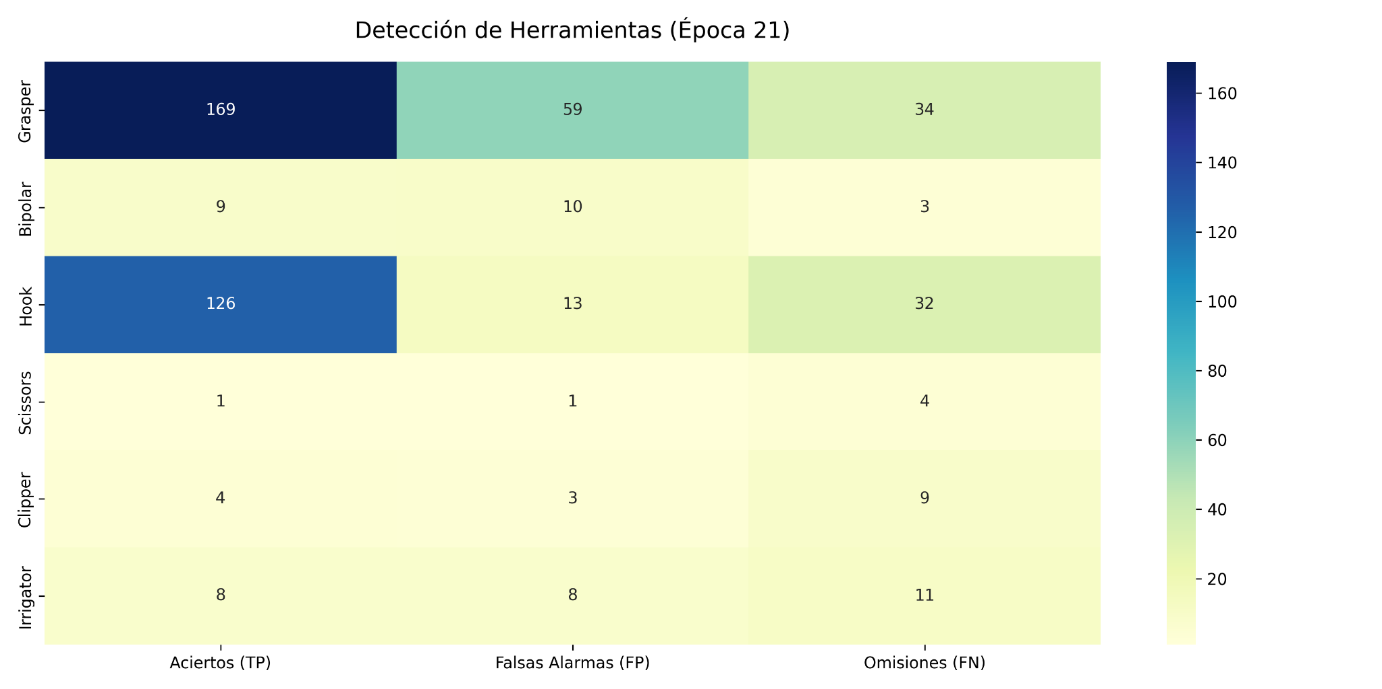
\includegraphics[width=\linewidth]{figures/fig04a_monolithic_ep21_instruments.png}
        \caption{Instrumentos}
    \end{subfigure}
    \par\bigskip
    \begin{subfigure}[b]{0.78\linewidth}
        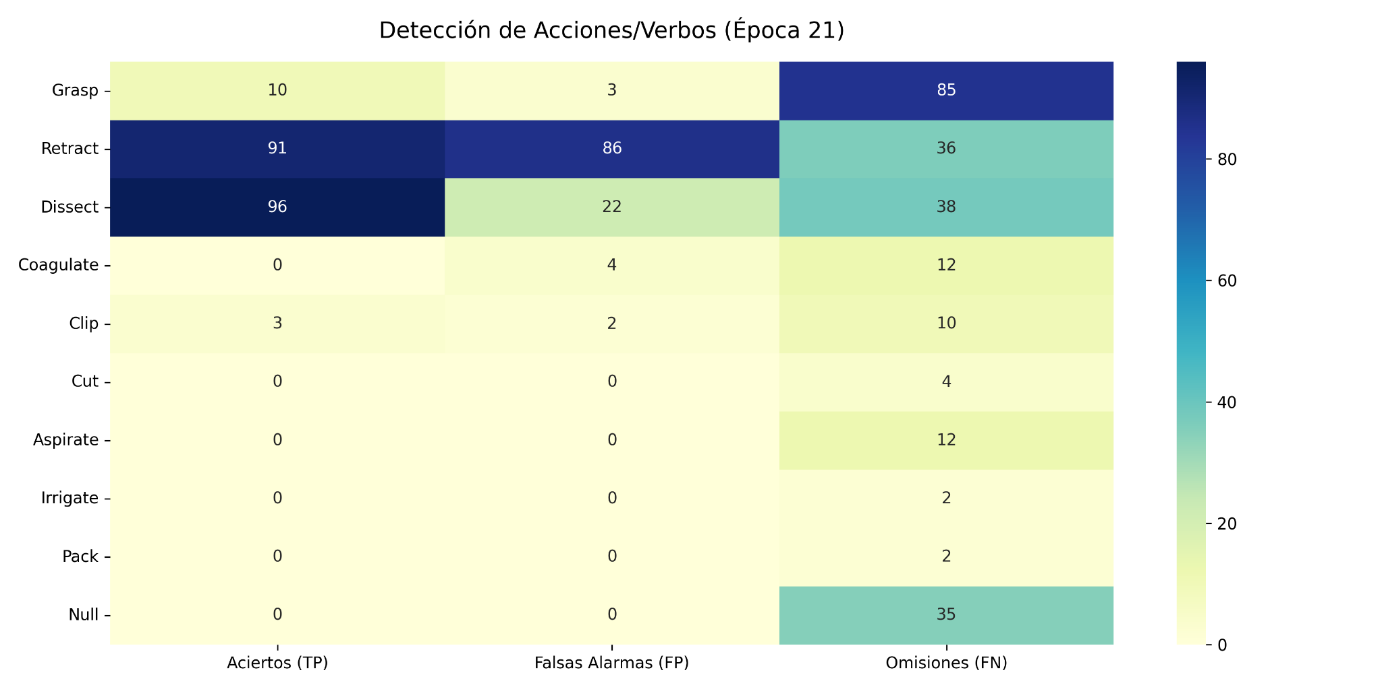
\includegraphics[width=\linewidth]{figures/fig04b_monolithic_ep21_verbs.png}
        \caption{Verbos}
    \end{subfigure}
    \par\bigskip
    \begin{subfigure}[b]{0.78\linewidth}
        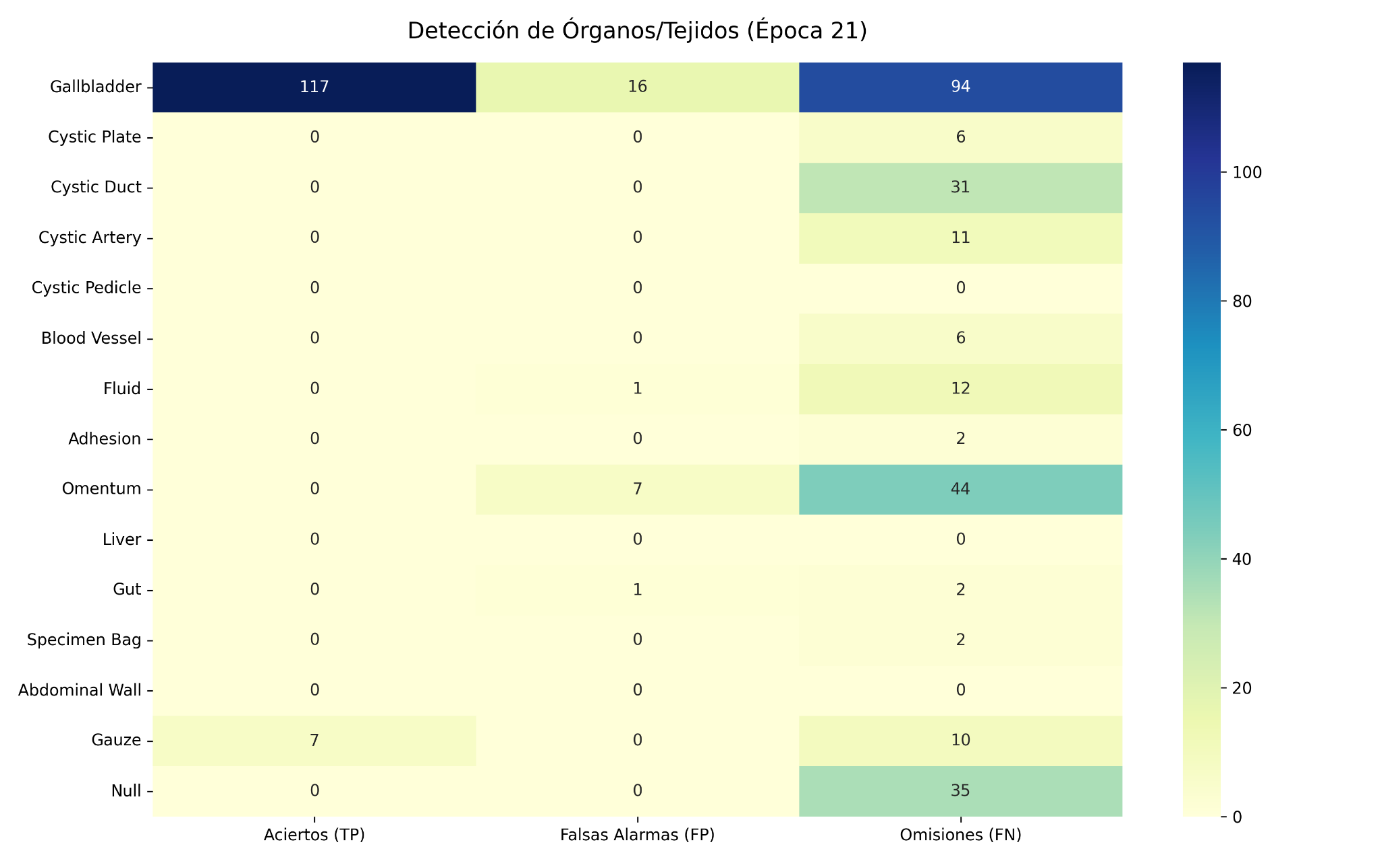
\includegraphics[width=\linewidth]{figures/fig04c_monolithic_ep21_organs.png}
        \caption{Órganos}
    \end{subfigure}
    \caption{Matrices de confusión multietiqueta del modelo monolítico en la Época~21: (a) instrumentos, (b) verbos, (c) órganos. Aprendizaje incipiente relativamente balanceado: 117 TP para vesícula biliar, 169 TP para Grasper.}
    \label{fig:monolithic-ep21}
\end{figure}

\begin{figure}[p]
    \centering
    \begin{subfigure}[b]{0.78\linewidth}
        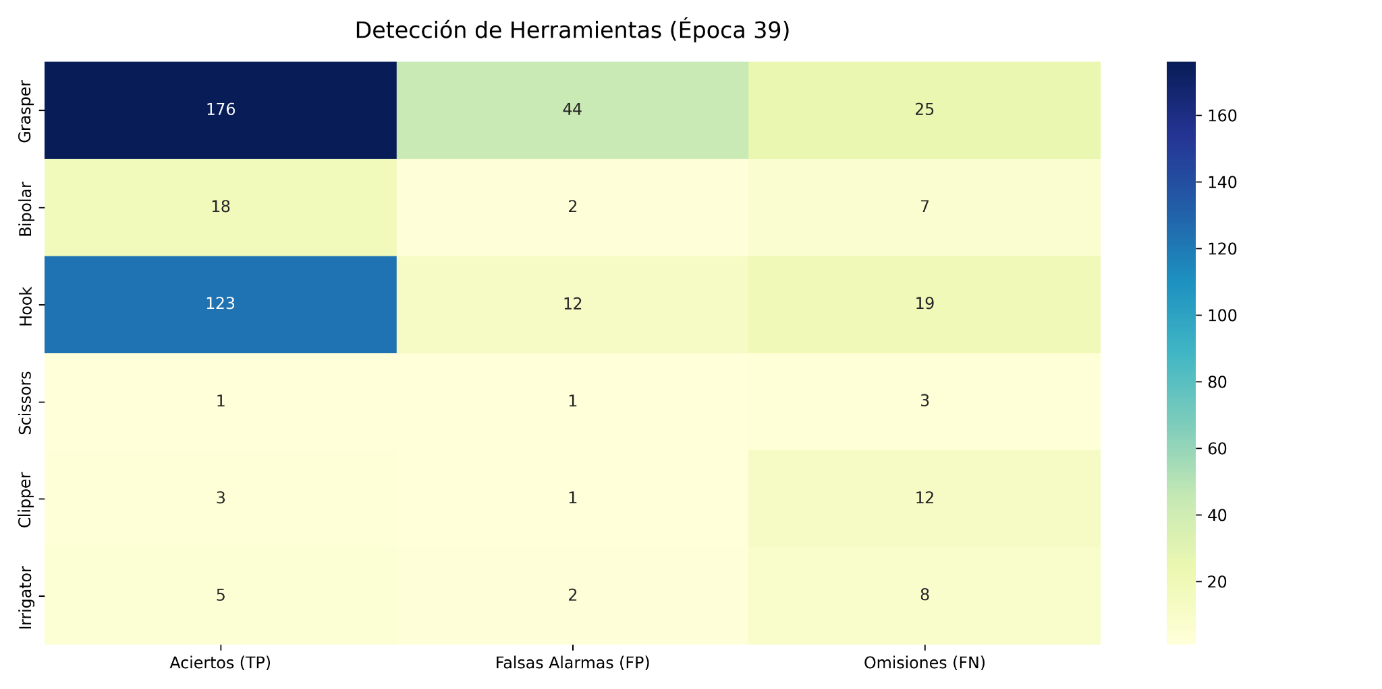
\includegraphics[width=\linewidth]{figures/fig05a_monolithic_ep39_instruments.png}
        \caption{Instrumentos}
    \end{subfigure}
    \par\bigskip
    \begin{subfigure}[b]{0.78\linewidth}
        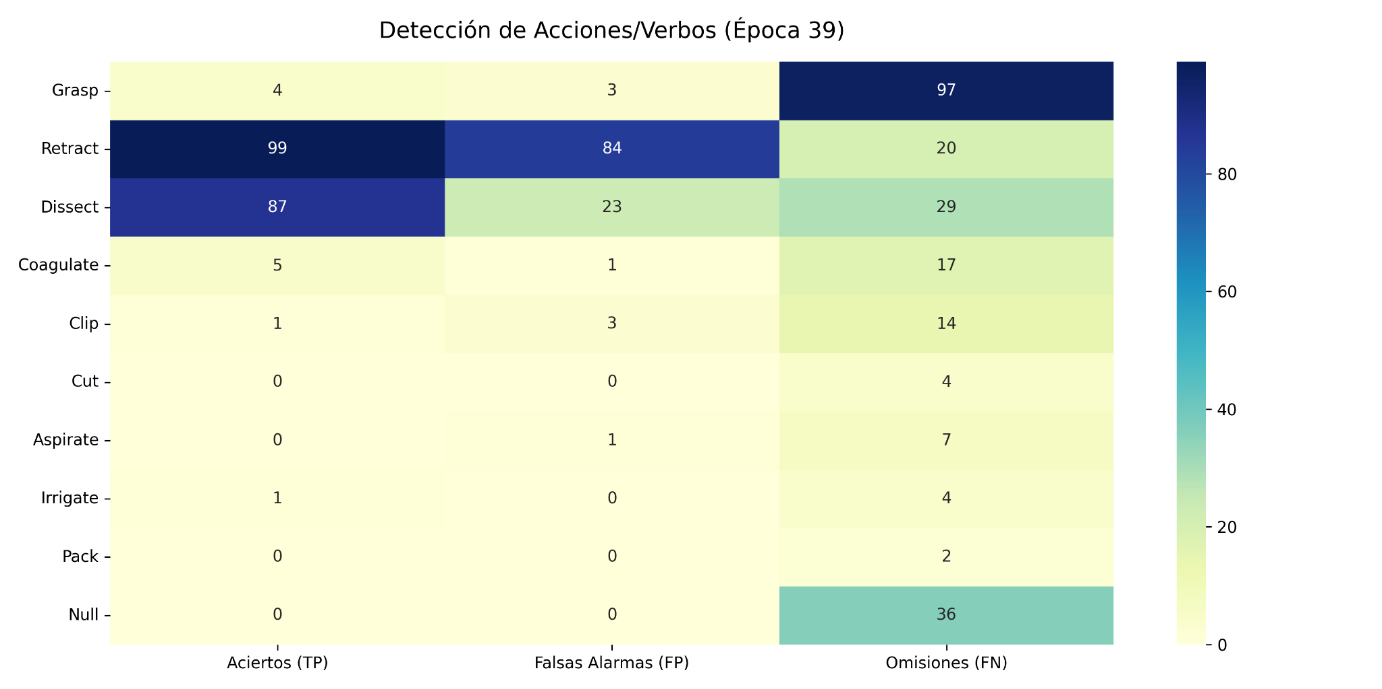
\includegraphics[width=\linewidth]{figures/fig05b_monolithic_ep39_verbs.png}
        \caption{Verbos}
    \end{subfigure}
    \par\bigskip
    \begin{subfigure}[b]{0.78\linewidth}
        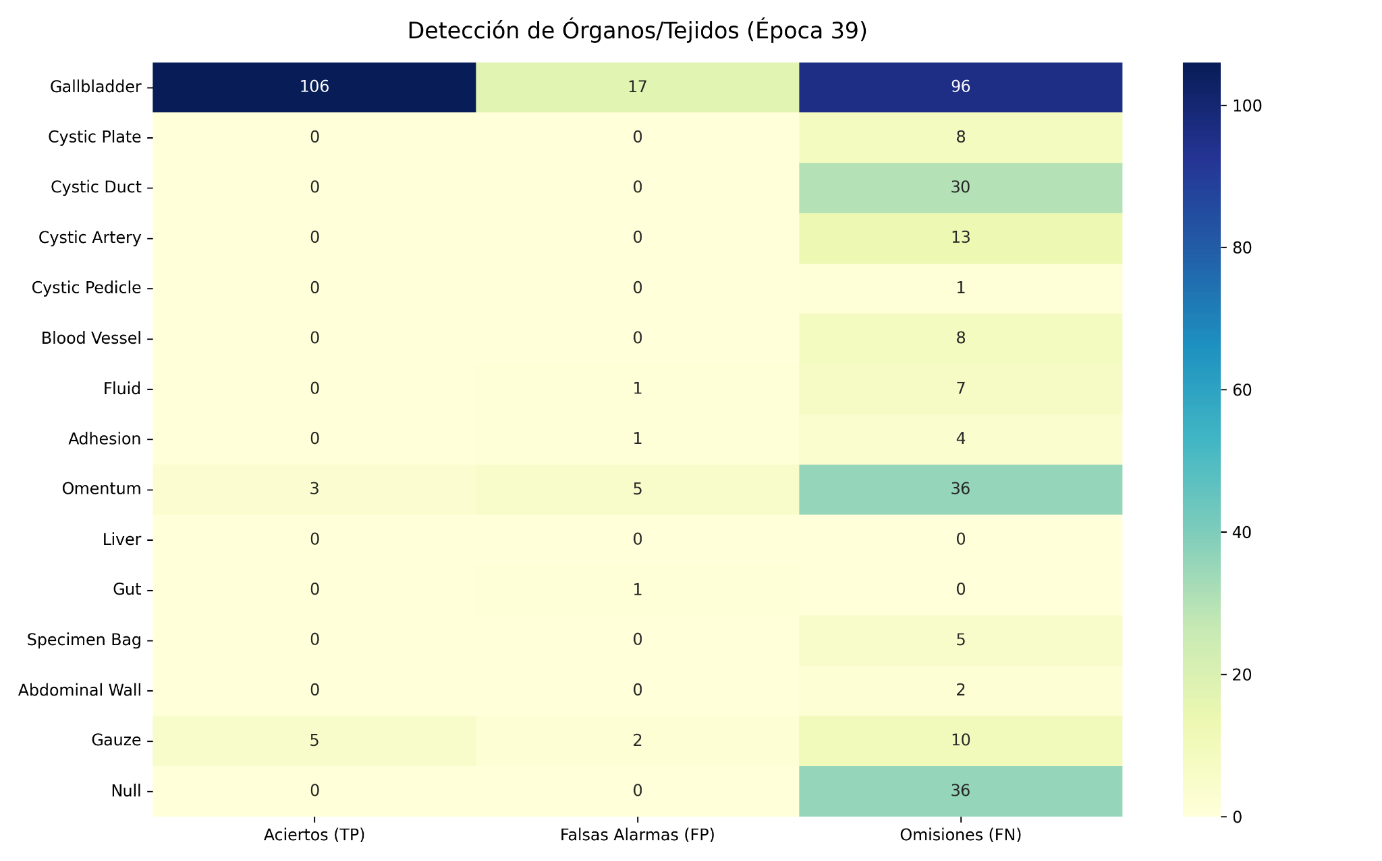
\includegraphics[width=\linewidth]{figures/fig05c_monolithic_ep39_organs.png}
        \caption{Órganos}
    \end{subfigure}
    \caption{Matrices de confusión multietiqueta del modelo monolítico en la Época~39. Tras 18 épocas adicionales, la rama de instrumentos mejora (176 TP para Grasper) mientras que la detección de órganos se degrada (la vesícula biliar cae a 106 TP con mayor número de omisiones). La asimetría confirma el diagnóstico de competencia de gradientes.}
    \label{fig:monolithic-ep39}
\end{figure}

\subsection{Especialización aislada}
\label{sec:resultados-especialistas}

Tras el diagnóstico del Horizonte~1, se implementó la estrategia de especialistas aislados: cada rama se entrenó de forma independiente con la ResNet-18 descongelada, permitiendo un ajuste fino específico por dominio semántico.

\subsubsection*{Especialista 1 — Instrumentos}

Con la ResNet-18 libre para actualizar sus pesos exclusivamente en función de la geometría y los reflejos metálicos de las herramientas quirúrgicas, el modelo logró un salto de rendimiento drástico. La \cref{tab:especialista-instrumentos} documenta su evolución.

\begin{table}[htbp]
    \centering
    \caption{Evolución del mAP\textsubscript{I} (\%) para el Especialista de Instrumentos aislado, con ResNet-18 descongelada. Punto de control óptimo: Época~6 con 86.42\,\%.}
    \label{tab:especialista-instrumentos}
    \small
    \begin{tabular}{@{}ccc@{}}
        \toprule
        \textbf{Época} & \textbf{Pérdida (Loss)} & \textbf{mAP\textsubscript{I} (\%)} \\
        \midrule
        0 & 0.2426 & 45.65 \\
        1 & 0.0728 & 75.92 \\
        2 & 0.0746 & 81.30 \\
        3 & 0.0348 & 83.79 \\
        4 & 0.1231 & 85.33 \\
        5 & 0.0426 & 85.37 \\
        6 & 0.4245 & \textbf{86.42} \\
        7 & 0.0205 & 85.18 \\
        \bottomrule
    \end{tabular}
\end{table}

Mientras que el entrenamiento monolítico requirió más de 40 épocas para estancarse en 60.09\,\%, el especialista aislado superó el 80\,\% en su segunda época y alcanzó un máximo de 86.42\,\% en la Época~6. Las matrices de confusión de la \cref{fig:especialista-instrumentos} —con 4{,}251 verdaderos positivos para \emph{Grasper} y 3{,}269 para \emph{Hook}— confirman que los mapas de activación generados por este módulo serán guías confiables para las ramas posteriores.

\begin{figure}[htbp]
    \centering
    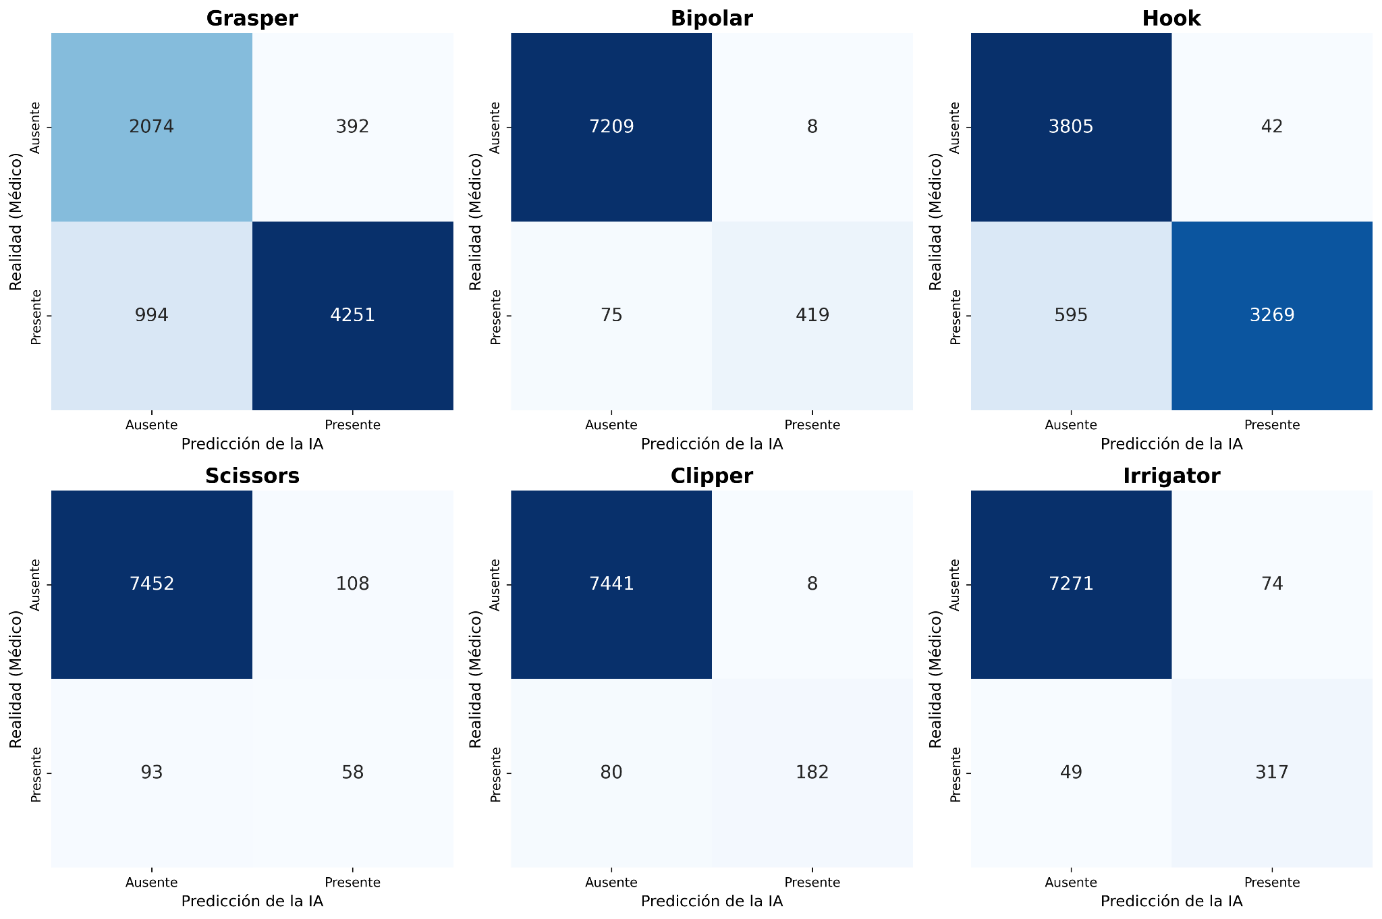
\includegraphics[width=0.92\linewidth]{figures/fig06_specialist_instruments_cm.png}
    \caption{Matrices de confusión binarias por clase para el Especialista de Instrumentos (Época~6, mAP: 86.42\,\%). Se observa una alta tasa de verdaderos positivos y una drástica reducción de falsas alarmas en herramientas críticas como \emph{Grasper} y \emph{Hook}.}
    \label{fig:especialista-instrumentos}
\end{figure}

\subsubsection*{Especialista 2 — Verbos (CAGAM)}

Las acciones quirúrgicas son eventos semánticos que ocurren en la interacción entre herramienta y tejido, sin bordes físicos evidentes. El módulo CAGAM aprovecha los mapas de activación del especialista de instrumentos para enfocar su análisis en las regiones espacialmente relevantes. La \cref{tab:especialista-verbos} documenta su evolución.

\begin{table}[htbp]
    \centering
    \caption{Evolución del mAP\textsubscript{V} (\%) para el Especialista de Verbos aislado (CAGAM). Se muestran los puntos de mayor incremento.}
    \label{tab:especialista-verbos}
    \small
    \begin{tabular}{@{}ccc@{}}
        \toprule
        \textbf{Época} & \textbf{Pérdida (Loss)} & \textbf{mAP\textsubscript{V} (\%)} \\
        \midrule
        0  & 0.1152 & 27.34 \\
        1  & 0.1532 & 38.49 \\
        4  & 0.1316 & 50.73 \\
        8  & 0.0740 & 52.04 \\
        14 & 0.0310 & \textbf{54.02} \\
        \bottomrule
    \end{tabular}
\end{table}

Al eliminar la interferencia de los gradientes anatómicos e instrumentales, el optimizador enfocó los pesos de la red puramente en la cinemática y posición de la herramienta. El modelo superó el 50\,\% de precisión en tan solo 4 épocas, alcanzando un máximo de \textbf{54.02\,\% en la Época~14}. Esto representa una mejora de más de 20 puntos porcentuales respecto al estancamiento en 33.06\,\% del enfoque monolítico.

\begin{figure}[htbp]
    \centering
    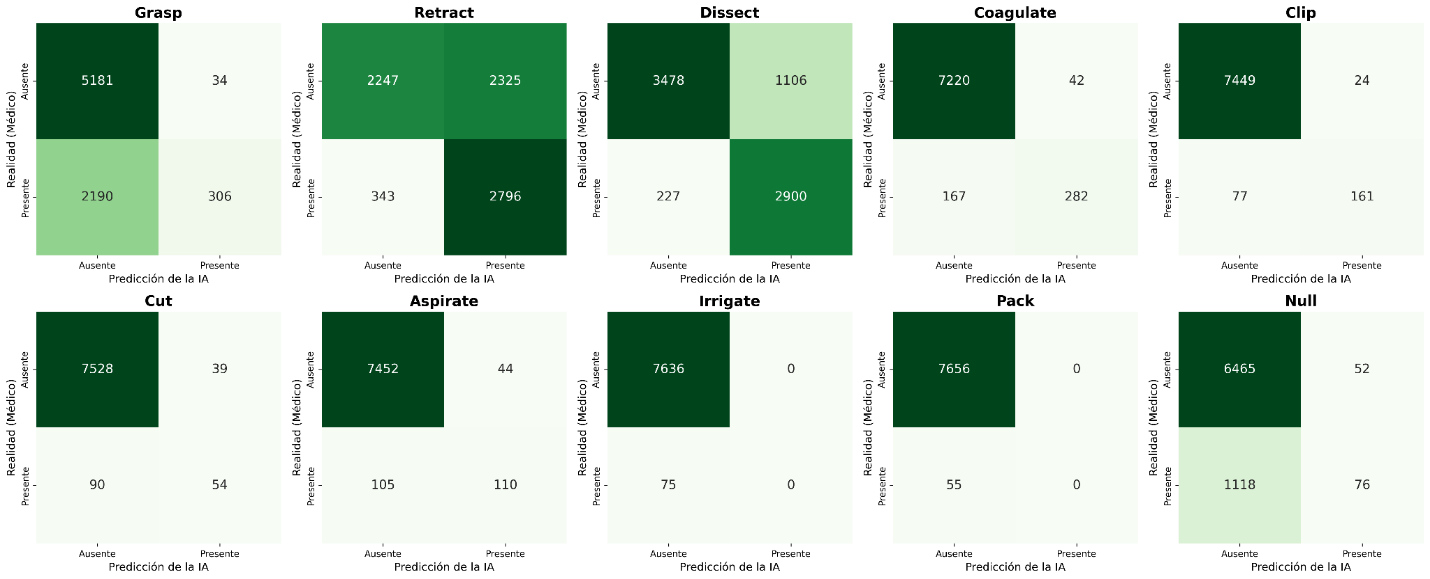
\includegraphics[width=\linewidth]{figures/fig07_specialist_verbs_cm.png}
    \caption{Matrices de confusión por clase para el Especialista de Verbos aislado (mAP\textsubscript{V}: 54.02\,\%). Se evidencia una sólida diagonal de verdaderos positivos en acciones de alta dependencia temporal como \emph{Retract}, \emph{Dissect} y \emph{Grasp}.}
    \label{fig:especialista-verbos}
\end{figure}

\subsubsection*{Especialista 3 — Órganos (T-CAM)}

La identificación de tejidos blandos representa el mayor reto de visión computacional en este dominio, debido a la alta deformabilidad de los órganos, la similitud de texturas y la variabilidad de la iluminación endoscópica. La \cref{tab:especialista-organos} resume su evolución.

\begin{table}[htbp]
    \centering
    \caption{Evolución del mAP\textsubscript{T} (\%) para el Especialista de Órganos aislado (T-CAM). Punto de control óptimo: Época~9 con 27.35\,\%.}
    \label{tab:especialista-organos}
    \small
    \begin{tabular}{@{}ccc@{}}
        \toprule
        \textbf{Época} & \textbf{Pérdida (Loss)} & \textbf{mAP\textsubscript{T} (\%)} \\
        \midrule
        0 & 0.2724 & 18.62 \\
        1 & 0.1285 & 25.77 \\
        3 & 0.2199 & 26.79 \\
        6 & 0.1326 & 27.01 \\
        8 & 0.1019 & 27.22 \\
        9 & 0.0883 & \textbf{27.35} \\
        \bottomrule
    \end{tabular}
\end{table}

Al liberar la retropropagación de la ResNet-18 exclusivamente para el dominio anatómico, el modelo rompió el bloqueo del Horizonte~1: experimentó un salto rápido en las primeras épocas, superando el límite previo del 19\,\% y estableciendo un nuevo máximo de \textbf{27.35\,\% en la Época~9}. Durante el entrenamiento monolítico, los aciertos para la vesícula biliar habían caído a 106 TP frente a 96 omisiones (FN); el especialista aislado logra 4{,}067 TP para la misma estructura, con mejoras también visibles en hígado (611 TP) y conducto cístico (250 TP).

\begin{figure}[htbp]
    \centering
    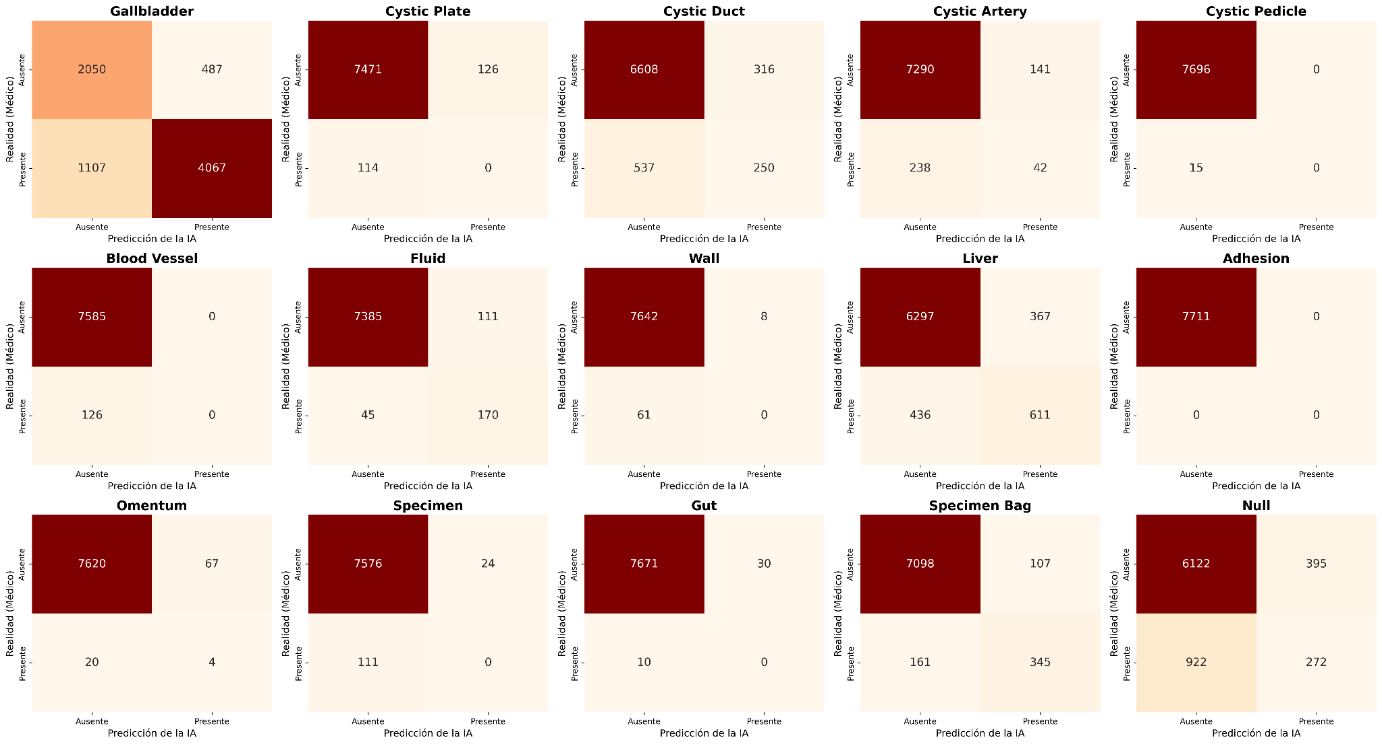
\includegraphics[width=0.85\linewidth]{figures/fig08_specialist_organs_cm.png}
    \caption{Matrices de confusión por clase para el Especialista de Órganos aislado (mAP\textsubscript{T}: 27.35\,\%). Se destaca la recuperación de la capacidad predictiva en estructuras clave como \emph{Gallbladder} y \emph{Liver}.}
    \label{fig:especialista-organos}
\end{figure}

\subsection{Fase de integración: fusión y co-adaptación extremo a extremo}
\label{sec:resultados-fusion}

La fase culminante consistió en inyectar los pesos pre-entrenados de los tres especialistas en una arquitectura RDV unificada y liberar la propagación de gradientes con una tasa de aprendizaje restrictiva. La \cref{tab:fusion} documenta la co-adaptación resultante.

\begin{table}[htbp]
    \centering
    \caption{Evolución del mAP (\%) de los componentes durante el ajuste fino de la fase de fusión.}
    \label{tab:fusion}
    \small
    \begin{tabular}{@{}ccccc@{}}
        \toprule
        \textbf{Época} & \textbf{mAP\textsubscript{I} (\%)} & \textbf{mAP\textsubscript{V} (\%)} & \textbf{mAP\textsubscript{T} (\%)} & \textbf{Promedio (\%)} \\
        \midrule
        0  & 36.95 & 28.05 & 9.60  & 24.87 \\
        10 & 71.00 & 44.31 & 13.95 & 43.08 \\
        15 & 73.57 & 45.44 & 15.46 & 44.82 \\
        19 & 76.34 & 47.07 & 17.34 & 46.92 \\
        21 & 76.33 & 46.49 & 19.60 & \textbf{47.49} \\
        \bottomrule
    \end{tabular}
\end{table}

En la Época~21, el Nodo de Rendezvous alcanzó una estabilidad que el enfoque monolítico no logró: un \textbf{promedio global de componentes del 47.49\,\%}. El modelo alcanzó un 53.4\,\% de AP en el Triplete~60 y un 35.3\,\% en el Triplete~82, indicando eficacia clínica en las interacciones quirúrgicas más comunes.

\begin{figure}[htbp]
    \centering
    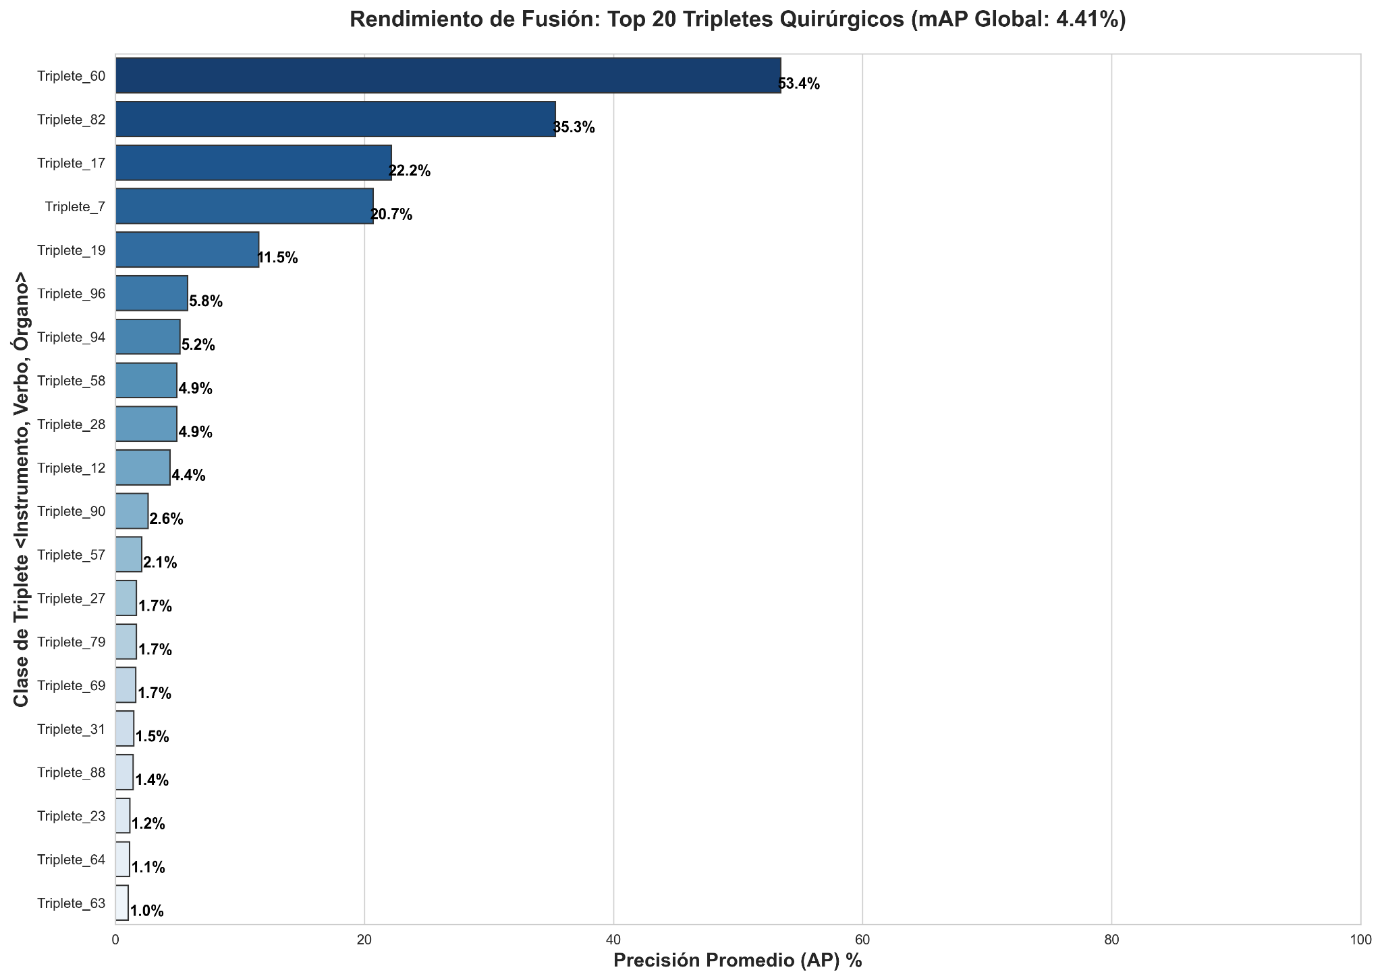
\includegraphics[width=\linewidth]{figures/fig09_fusion_top20_triplets.png}
    \caption{Rendimiento predictivo de la fase de fusión. Top 20 de tripletes quirúrgicos con mayor AP. El mAP\textsubscript{IVT} global de 4.41\,\% refleja la penalización combinatoria del espacio de 100 clases con distribución fuertemente sesgada.}
    \label{fig:fusion-top20}
\end{figure}

\subsection{Diagnóstico matemático y corrección de activaciones en la fusión}
\label{sec:diagnostico-matematico}

Durante las primeras iteraciones de la fase de integración espaciotemporal, el modelo experimentó un estancamiento analítico severo. La función de pérdida (\emph{BCEWithLogitsLoss}) convergía tempranamente a un valor constante de $\ln(2) \approx 0.693$. Matemáticamente, este valor corresponde a la pérdida esperada cuando la red asigna una probabilidad de 0.5 a todas las clases independientemente de la entrada, lo que equivale a predicción aleatoria:

\begin{equation}
    \mathcal{L}_{\text{BCE}} = -\big[y \cdot \log(0.5) + (1-y) \cdot \log(0.5)\big] = -\log(0.5) = \log(2) \approx 0.693
    \label{eq:bce}
\end{equation}

El diagnóstico profundo de la topología y el flujo de tensores reveló dos deficiencias estructurales críticas:

\begin{itemize}[leftmargin=1.4em]
    \item \textbf{Truncamiento de gradientes negativos (el problema espacial).} El módulo de refinamiento contaba con una función de activación ReLU en su capa de salida. Las representaciones espaciales (CAMs) emiten activaciones fuertemente negativas (p.\,ej., $< -6.0$) en regiones donde existe certeza de ausencia de un instrumento u órgano. Al pasar por ReLU, estos valores se truncaban a cero, destruyendo la certeza restrictiva de la red. Al retirar esta activación final, los gradientes negativos recuperaron su flujo causal.
    \item \textbf{Logits de baja magnitud en la TCN (el problema temporal).} Los logits crudos emitidos por la TCN poseían un rango dinámico estrecho. Al ser evaluados directamente, generaban factores de atención cercanos a $0.5$, actuando como un simple filtro de opacidad en lugar de una compuerta lógica restrictiva. Mediante la calibración de estos tensores temporales y la normalización de las CAMs extraídas por video, $(x - \mu)/\sigma$, se obligó al sistema a emitir decisiones polares (confianza cercana al 0\,\% o al 100\,\%), reactivando el aprendizaje diferencial.
\end{itemize}

\subsection{Comparativa con el estado del arte}
\label{sec:comparativa}

\textbf{Nota metodológica.} Las dos implementaciones locales (RDV Local y SpatioTemporalRDV) se evaluaron sobre los mismos 9 videos del Fold~1 de validación cruzada, por lo que su comparación directa es válida. La columna ``RDV Original'' reporta el promedio de validación cruzada de 5 \emph{folds} sobre CholecT50 con infraestructura multi-GPU; dado que el presente trabajo evalúa un solo \emph{fold} en hardware de consumo, dicha columna sirve únicamente como referencia orientativa y no constituye una comparación de equivalencia estadística. Para evitar lecturas erróneas, esta columna se presenta sombreada y en cursiva en la \cref{tab:comparativa}.

\begin{table}[htbp]
    \centering
    \caption{Comparativa directa entre el modelo Rendezvous original \cite{nwoye2022rendezvous} y las implementaciones desarrolladas en este proyecto.}
    \label{tab:comparativa}
    \small
    \begin{tabular}{@{}lccc@{}}
        \toprule
        \textbf{Métrica} & \cellcolor{gray!15}\textit{RDV Original\textsuperscript{\dag}} & \textbf{RDV Local} & \textbf{SpatioTemporalRDV} \\
        \midrule
        mAP\textsubscript{I} (\%)   & \cellcolor{gray!15}\textit{92.0} & 70.78 & \textbf{77.56} \\
        mAP\textsubscript{V} (\%)   & \cellcolor{gray!15}\textit{60.7} & 48.70 & \textbf{53.59} \\
        mAP\textsubscript{T} (\%)   & \cellcolor{gray!15}\textit{38.3} & 18.10 & \textbf{38.45} \\
        mAP\textsubscript{IVT} (\%) & \cellcolor{gray!15}\textit{29.9} & 2.06  & \textbf{13.38} \\
        Hardware requerido & \cellcolor{gray!15}\textit{Clúster multi-GPU} & \multicolumn{2}{c}{GTX 1050 (3\,GB)} \\
        \bottomrule
    \end{tabular}

    \vspace{0.4em}
    {\footnotesize \textsuperscript{\dag} Los valores del RDV Original corresponden al promedio de validación cruzada de 5 \emph{folds} sobre CholecT50 con infraestructura multi-GPU \cite{nwoye2022rendezvous}. La comparación directa con las implementaciones locales es orientativa.}
\end{table}

Los resultados de la \cref{tab:comparativa} evidencian una drástica evolución arquitectónica al incorporar el eje temporal. A continuación, el análisis por dominio semántico.

\subsubsection*{I. Herramientas (dominio espacial)}

La rama de instrumentos incrementó su mAP\textsubscript{I} a 77.56\,\%. El contexto temporal permitió al sistema exigir coherencia de trayectoria, reduciendo las detecciones espurias de instrumentos presentes en un solo fotograma.

\begin{figure}[htbp]
    \centering
    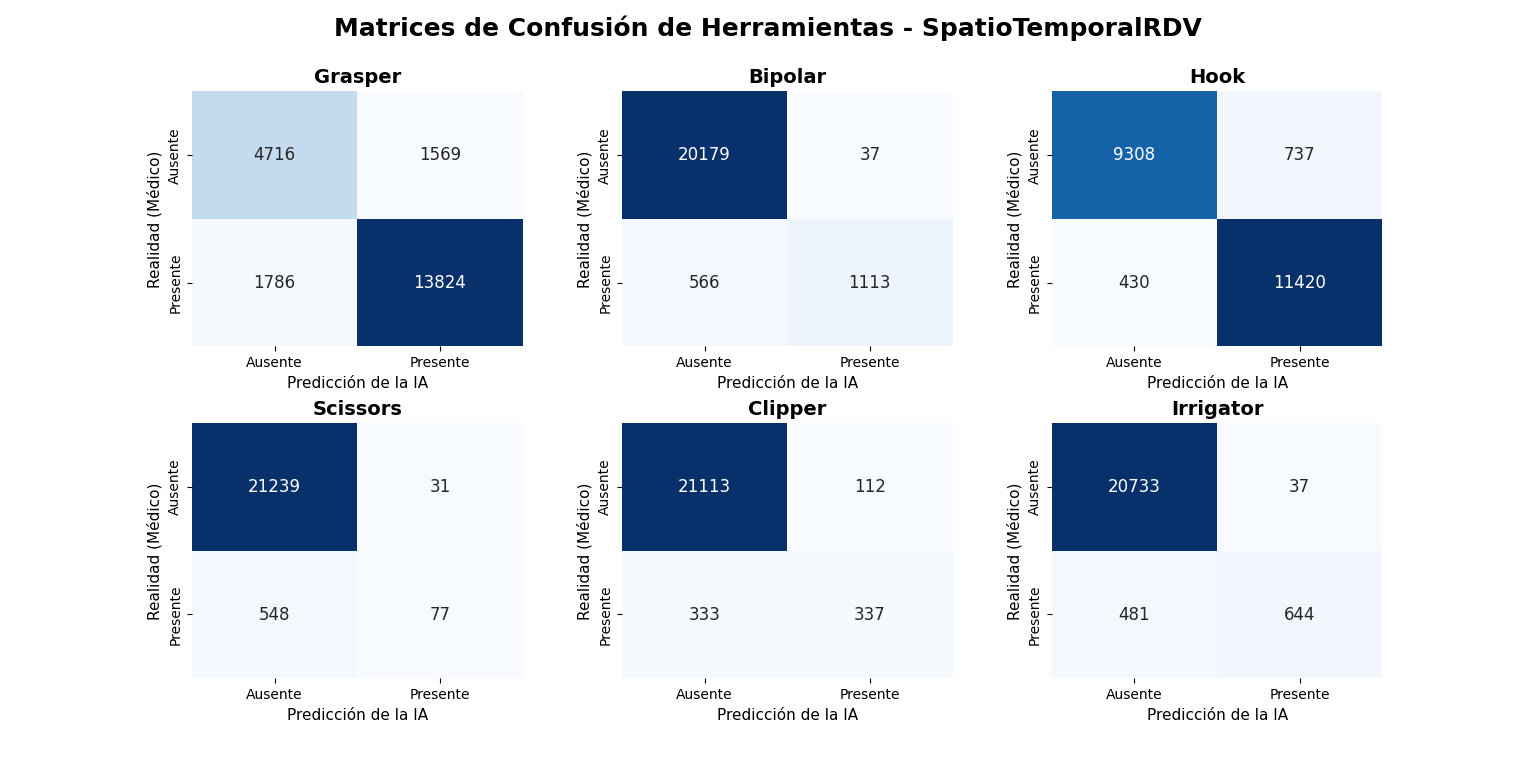
\includegraphics[width=0.9\linewidth]{figures/fig10_spatiotemporal_instruments_cm.png}
    \caption{Matrices de confusión binarias por clase para la detección de herramientas del modelo SpatioTemporalRDV.}
    \label{fig:st-instrumentos}
\end{figure}

\subsubsection*{II. Acciones quirúrgicas}

El mAP\textsubscript{V} alcanzó el 53.59\,\%. Las acciones de alta dependencia cinemática —\emph{Retract}, \emph{Dissect}— muestran las mejoras más pronunciadas, confirmando la contribución de la ventana temporal de 17 fotogramas de la TCN.

\begin{figure}[htbp]
    \centering
    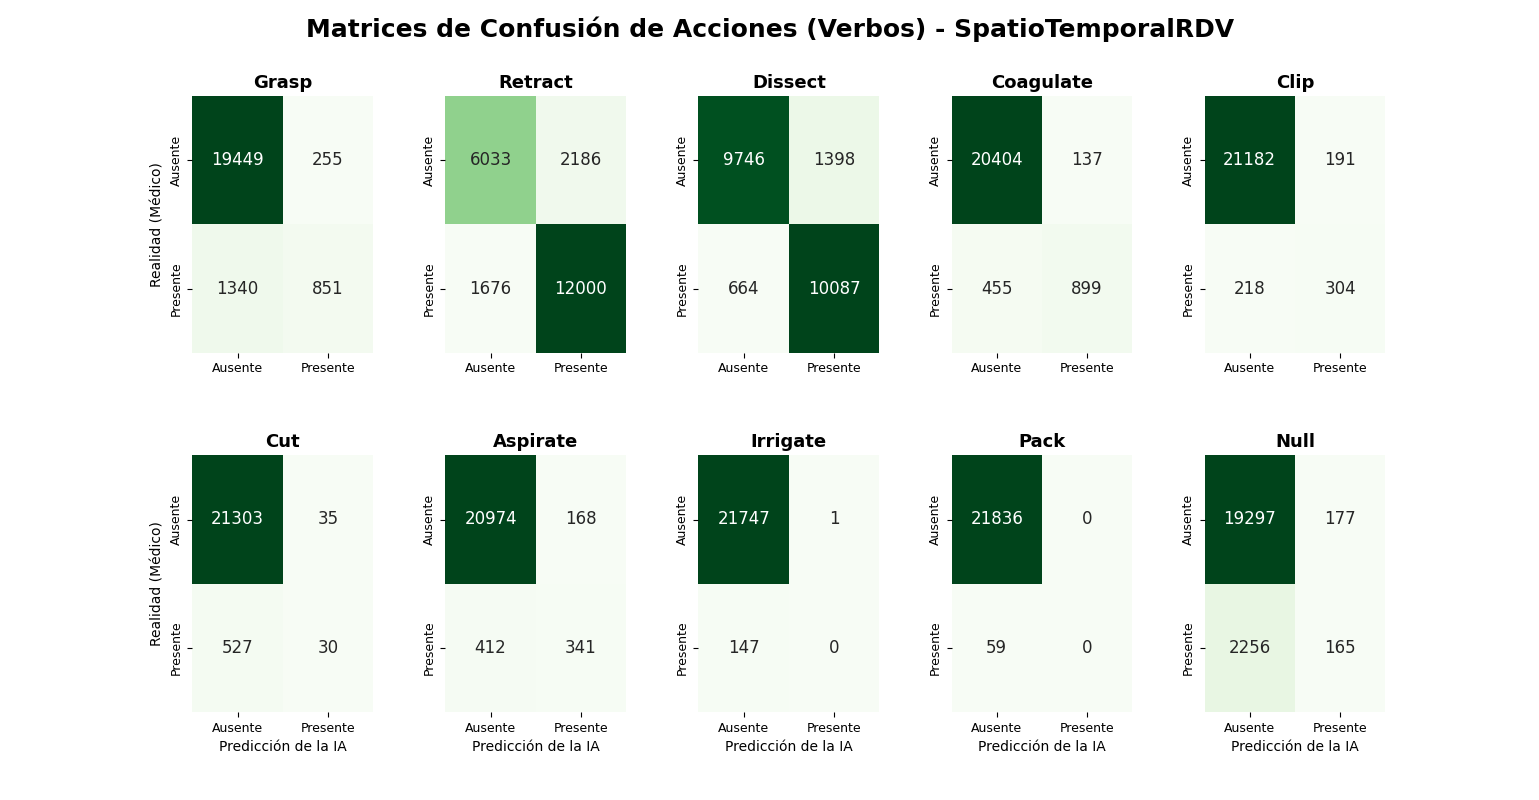
\includegraphics[width=\linewidth]{figures/fig11_spatiotemporal_verbs_cm.png}
    \caption{Matrices de confusión para las 10 clases de verbos. Se aprecia la capacidad de la TCN para discernir acciones de alta dependencia temporal.}
    \label{fig:st-verbos}
\end{figure}

\subsubsection*{III. Resolución del problema anatómico (dominio de tejidos)}

El mayor avance técnico reside en la inferencia de órganos blandos. El modelo espaciotemporal duplicó el mAP\textsubscript{T} estático (de 18.10\,\% a 38.45\,\%), cerrando prácticamente la brecha con el valor de referencia reportado por Nwoye et al. (38.3\,\%) \cite{nwoye2022rendezvous}. Este resultado indica que la integración temporal mitigó de forma efectiva el ``mar rosa'' al proveer contexto de trayectoria y persistencia estructural. No obstante, dado que la comparación con el valor de referencia involucra diferentes protocolos de evaluación, el resultado debe interpretarse como evidencia empírica favorable a la hipótesis de aislamiento de gradientes, y no como superación demostrada del estado del arte.

\begin{figure}[htbp]
    \centering
    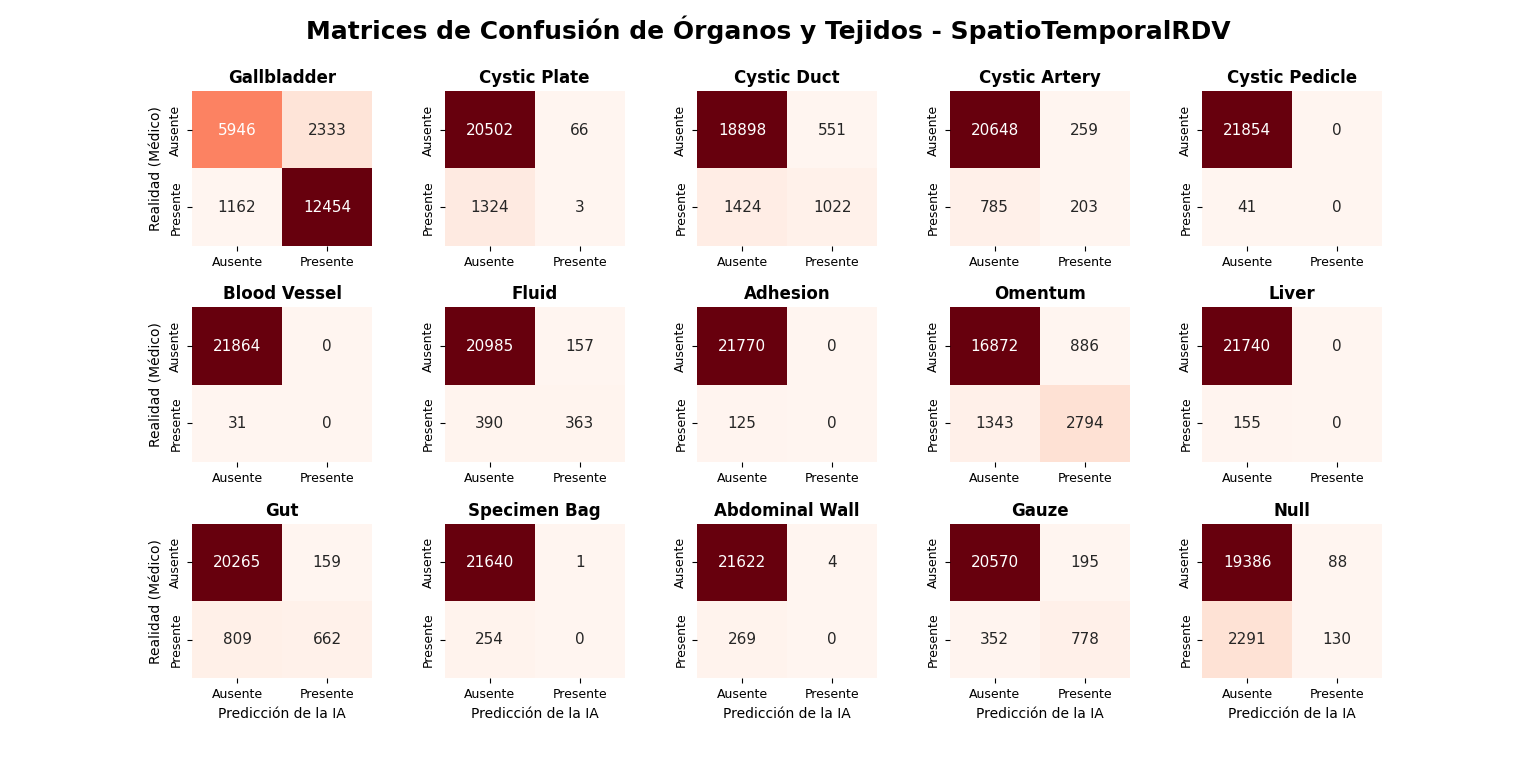
\includegraphics[width=0.88\linewidth]{figures/fig12_spatiotemporal_organs_cm.png}
    \caption{Matrices de confusión para la detección de tejidos y órganos del modelo SpatioTemporalRDV.}
    \label{fig:st-organos}
\end{figure}

\subsubsection*{IV. Evaluación holística: el triplete quirúrgico}

La predicción conjunta escaló de 2.06\,\% a 13.38\,\% de mAP\textsubscript{IVT}, un incremento de 6.5 veces respecto a la variante estática local. Debe contextualizarse que el \emph{baseline} local (2.06\,\%) es considerablemente inferior al reportado en el trabajo original (29.9\,\%), debido a las restricciones de hardware, la evaluación sobre un solo \emph{fold} y la ausencia de técnicas de aumento de datos sobre clases de baja frecuencia. El análisis de los 20 tripletes más frecuentes (\cref{fig:st-top20}) muestra picos de AP superiores al 80\,\% para combinaciones fundamentales de la colecistectomía laparoscópica.

\begin{figure}[htbp]
    \centering
    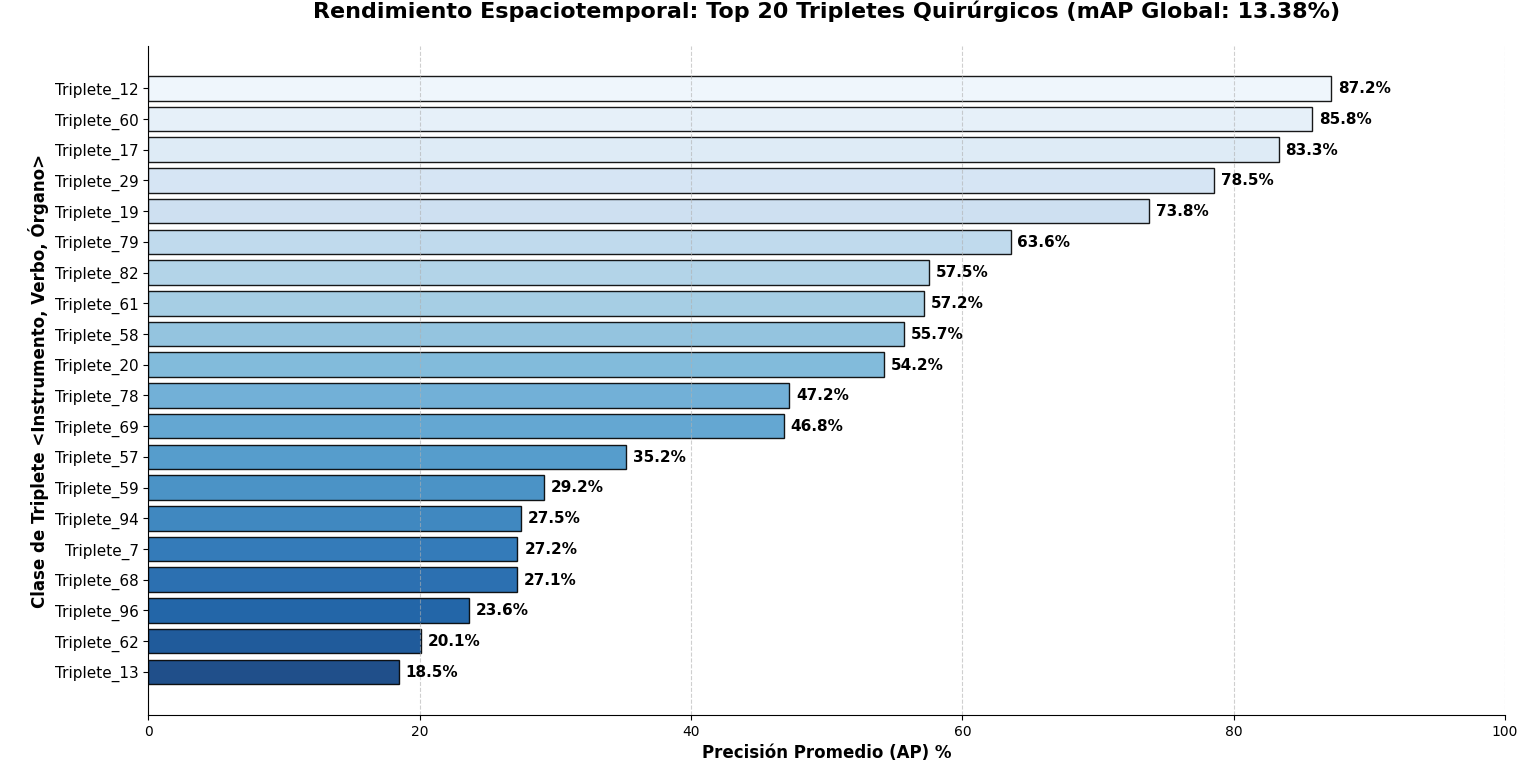
\includegraphics[width=\linewidth]{figures/fig13_spatiotemporal_top20_triplets.png}
    \caption{Rendimiento predictivo holístico. Top 20 de tripletes quirúrgicos con mayor Precisión Promedio (AP) evaluados bajo la arquitectura SpatioTemporalRDV.}
    \label{fig:st-top20}
\end{figure}

\section{Discusión}
\label{sec:discusion}

\subsection{Síntesis e interpretación de los resultados}
\label{sec:sintesis}

El hilo conductor de los tres horizontes de desarrollo es una única hipótesis: el estancamiento del entrenamiento monolítico en \cref{sec:resultados-monolitico} no era un problema de capacidad del modelo, sino de \textbf{competencia de gradientes} entre dominios semánticos con distinta escala de magnitud de error. Esta hipótesis se sostiene sobre tres líneas de evidencia convergentes. Primero, la asimetría observada en la Tabla~\ref{tab:monolitico} —instrumentos mejorando mientras los órganos permanecen esencialmente congelados— es la firma característica de un gradiente dominante que satura la actualización de pesos compartidos. Segundo, al desacoplar el entrenamiento en especialistas independientes (\cref{sec:resultados-especialistas}), el AP anatómico se recuperó de 19.52\,\% a 27.35\,\% sin ningún otro cambio arquitectónico más que la eliminación de la interferencia entre ramas. Tercero, la fase de fusión (\cref{sec:resultados-fusion}) demostró que esta ganancia no era artefacto de sobreajuste al aislamiento: los tres componentes co-adaptaron exitosamente hasta un promedio de 47.49\,\%, muy por encima del techo monolítico.

Conviene ser precisos sobre el alcance causal de esta interpretación. El aislamiento modular fue la intervención introducida, pero se acompañó simultáneamente del descongelamiento de la ResNet-18 para cada especialista, un cambio que por sí mismo también incrementa la capacidad de ajuste. Sin un \emph{ablation study} formal que mantenga el descongelamiento fijo y solo varíe el aislamiento —o viceversa—, la mejora observada debe leerse como evidencia consistente con la hipótesis de competencia de gradientes, y no como una demostración aislada de causalidad; este punto se retoma en la \cref{sec:limitaciones} y se propone como la prioridad inmediata del trabajo futuro (\cref{sec:trabajo-futuro}).

La integración espaciotemporal aporta una segunda lectura relevante: el salto de mAP\textsubscript{IVT} de 2.06\,\% a 13.38\,\% (6.5$\times$) al incorporar la TCN indica que buena parte de la señal semántica de los tripletes quirúrgicos —particularmente en verbos como \emph{Retract} y \emph{Dissect}— es inherentemente temporal y no puede extraerse de manera confiable desde un análisis estático fotograma a fotograma. Esto es coherente con la intuición clínica de que una acción quirúrgica se define por su cinemática, no por una postura instantánea.

\subsection{Comparación con la literatura y significado práctico}
\label{sec:comparacion-literatura}

La motivación original de este trabajo —expuesta en la \cref{sec:contexto}— fue habilitar el reconocimiento automático de tripletes quirúrgicos fuera de la infraestructura de clúster multi-GPU típicamente empleada en la literatura \cite{nwoye2022rendezvous,twinanda2017}. En ese sentido, el resultado más significativo no es únicamente cuantitativo, sino metodológico: la variante SpatioTemporalRDV alcanzó un mAP\textsubscript{T} de 38.45\,\%, próximo al valor de referencia de 38.3\,\% reportado por Nwoye et al. \cite{nwoye2022rendezvous}, evaluada íntegramente en un equipo portátil con 3~GB de VRAM. Este acercamiento en el dominio anatómico —el más difícil por el problema del ``mar rosa'' (\cref{sec:problematica})— sugiere que la estrategia de especialización aislada seguida de fusión es una alternativa viable al entrenamiento extremo a extremo cuando el hardware es el factor limitante, sin necesidad de simplificar la arquitectura de atención de dos niveles que caracteriza al modelo original.

Al mismo tiempo, la brecha en mAP\textsubscript{IVT} (13.38\,\% frente al 29.9\,\% de referencia) muestra que el triplete completo —la tarea combinatoria más exigente, con 100 clases y distribución fuertemente sesgada— sigue beneficiándose de manera desproporcionada de la validación cruzada completa, el mayor volumen efectivo de datos de entrenamiento y las técnicas de aumento de datos que la infraestructura multi-GPU permite. En términos prácticos, esto sitúa la contribución del presente trabajo no como un reemplazo del entrenamiento a gran escala, sino como una vía de acceso metodológico: una ruta para que grupos de investigación con recursos computacionales limitados puedan explorar, diagnosticar y prototipar variantes de la arquitectura Rendezvous antes de escalarlas a infraestructura mayor.

\subsection{Limitaciones del estudio}
\label{sec:limitaciones}

Las siguientes limitaciones son inherentes al alcance y a las restricciones de hardware del proyecto, y delimitan la interpretación de los resultados anteriores:

\begin{enumerate}[leftmargin=1.6em]
    \item \textbf{Evaluación sobre un solo \emph{fold}.} Todos los resultados cuantitativos corresponden al Fold~1 del protocolo de validación cruzada de 5 \emph{folds}. La varianza entre \emph{folds} puede ser significativa; una evaluación completa requeriría 5 ejecuciones independientes, que excedieron el alcance temporal y computacional del servicio social.
    \item \textbf{Ausencia de \emph{ablation study} formal.} La arquitectura evolucionó en tres horizontes, pero no se realizaron experimentos de ablación controlados (por ejemplo, fusión sin TCN, o modelo monolítico con ResNet-18 descongelada). Por lo tanto, la contribución individual de cada componente metodológico no puede atribuirse causalmente de forma aislada con los datos disponibles.
    \item \textbf{Reproducibilidad parcial.} La semilla aleatoria 42 se fijó explícitamente en las operaciones de partición del módulo de fusión y la TCN. No se verificó el fijado de semilla en las capas internas del entrenamiento de especialistas, por lo que pequeñas variaciones entre corridas son posibles.
    \item \textbf{Campo receptivo fijo de la TCN.} La TCN implementada cubre un campo receptivo de 17 fotogramas. Dependencias temporales de rango mayor (p.\,ej., fases quirúrgicas de varios minutos) quedan fuera del alcance del modelo actual.
    \item \textbf{Ajuste fino no completamente extremo a extremo.} La estrategia de extracción fuera de línea congela el \emph{backbone} durante el entrenamiento del módulo de fusión, impidiendo la co-adaptación completa del extractor de características con la cabeza de fusión.
    \item \textbf{Varianza entre corridas no cuantificada.} Todos los resultados reportados corresponden a una sola ejecución por configuración. Aunque el módulo de fusión y la TCN sí tienen semilla aleatoria fijada, no se realizaron corridas adicionales con semillas distintas para estimar la varianza del entrenamiento; por lo tanto, diferencias como la mejora de puntos porcentuales entre horizontes no distinguen formalmente señal de ruido de inicialización.
\end{enumerate}

En conjunto, estas limitaciones no invalidan el patrón observado —la asimetría sistemática entre instrumentos y órganos bajo entrenamiento monolítico, y su reversión bajo aislamiento, es demasiado grande y consistente para atribuirse a ruido de una sola corrida—, pero sí acotan la fuerza de las afirmaciones causales y comparativas que pueden derivarse de este trabajo hasta que se completen la validación cruzada de 5 \emph{folds} y el \emph{ablation study} formal.

\section{Conclusiones}
\label{sec:conclusiones}

La investigación y desarrollo realizada demostró la viabilidad de implementar, optimizar y adaptar la arquitectura Rendezvous para el reconocimiento de tripletes quirúrgicos bajo restricciones severas de hardware. A través del análisis evolutivo de los tres horizontes de desarrollo, se extraen las siguientes conclusiones fundamentales:

\begin{enumerate}[leftmargin=1.6em]
    \item \textbf{Evidencia de mitigación de la competencia de gradientes mediante aislamiento modular} (causa no aislada de otros factores). El entrenamiento monolítico con hardware limitado colapsó por la dominancia de los gradientes de instrumentos sobre los anatómicos, estancando el AP de órganos en 19.52\,\%. La estrategia de especialistas aislados demostró ser matemáticamente superior: el AP anatómico escaló a 27.35\,\% y el de instrumentos a 86.42\,\%, validando empíricamente el diagnóstico de competencia de gradientes. La contribución específica del aislamiento respecto a otros factores (descongelamiento del \emph{backbone}, hiperparámetros) no puede determinarse sin un \emph{ablation study} formal, lo que constituye una línea de trabajo futuro inmediata.

    \item \textbf{Preservación del mecanismo de atención condicionada} (CAGAM y T-CAM). La separación modular no destruyó la premisa central de la arquitectura: la atención espacial condicionada. Al entrenar primero al especialista de instrumentos, los módulos posteriores recibieron mapas de atención precisos. El salto en la detección de acciones complejas —superando el 54\,\% de mAP\textsubscript{V}— confirma que la red replica el comportamiento del modelo original a una fracción del costo computacional.

    \item \textbf{Viabilidad del entrenamiento en hardware de consumo.} Este proyecto propone un \emph{pipeline} metodológico que permite alcanzar la fase de fusión utilizando hardware de consumo (Lenovo IdeaPad Gaming). La inyección de pesos pre-entrenados y la tasa de aprendizaje restrictiva posibilitaron la co-adaptación final sin exceder la memoria VRAM disponible, abriendo la puerta a la investigación en este dominio fuera de clústeres multi-GPU, con las limitaciones de protocolo ya señaladas en la \cref{sec:limitaciones}.

    \item \textbf{Contribución de la integración temporal y límites del sistema.} La arquitectura SpatioTemporalRDV multiplicó por 6.5 el mAP\textsubscript{IVT} de la variante estática local (2.06\,\% $\rightarrow$ 13.38\,\%) y alcanzó un mAP\textsubscript{T} de 38.45\,\%, próximo al valor de referencia de Nwoye et al. \cite{nwoye2022rendezvous} (38.3\,\%), aunque obtenido bajo un protocolo de evaluación menos riguroso. Alcanzar la frontera del 29.9\,\% en mAP\textsubscript{IVT} requeriría infraestructura multi-GPU, validación cruzada completa de 5 \emph{folds}, técnicas de aumento de datos para clases de baja frecuencia, y un \emph{ablation study} que permita optimizar la arquitectura de forma controlada.
\end{enumerate}

\section{Trabajo futuro}
\label{sec:trabajo-futuro}

El éxito de la arquitectura SpatioTemporalRDV abre líneas de investigación directas. En el corto plazo, la prioridad técnica es completar el \emph{ablation study} formal para aislar la contribución de cada componente (TCN, descongelamiento del \emph{backbone}, aislamiento de gradientes) y ejecutar la \textbf{validación cruzada completa de 5 \emph{folds}} para obtener métricas estadísticamente comparables con la literatura.

En el mediano plazo, las representaciones aprendidas constituyen el cimiento ideal para una \textbf{arquitectura generativa} capaz de sintetizar video quirúrgico artificial. Si bien el modelo desarrollado en este proyecto es de naturaleza estrictamente discriminativa (optimizado para modelar la probabilidad condicional $P(Y\mid X)$ y clasificar eventos existentes), sus representaciones matemáticas podrían reutilizarse como señal de condicionamiento para un modelo generativo (modelando $P(X\mid Y)$).

Para lograr la generación condicionada de secuencias de video realistas —por ejemplo, ante una solicitud del usuario como ``generar un clip de la acción \emph{Retract} con un \emph{Grasper} sobre la vesícula''—, se propone la siguiente transición arquitectónica como trabajo futuro. Esta propuesta se enmarca en una línea de investigación activa y no exploratoria desde cero: trabajos recientes ya han demostrado la viabilidad de la síntesis de video quirúrgico mediante modelos de difusión condicionados por texto o por instrumentos \cite{cho2024surgen}, y específicamente sobre cirugía laparoscópica con arquitecturas de difusión interactivas \cite{iliash2025interactive}. La contribución potencial de este proyecto sería condicionar dicha síntesis con las señales semánticas de tripletes (instrumento-verbo-órgano) extraídas por SpatioTemporalRDV, en lugar de únicamente texto:

\begin{itemize}[leftmargin=1.4em]
    \item \textbf{Codificador semántico (condicionamiento).} La red SpatioTemporalRDV actual se mantendría con sus pesos congelados, operando como el ``cerebro semántico'' del sistema. En lugar de clasificar, sus mapas de atención 2D y sus vectores temporales se utilizarían como ``instrucciones matemáticas'' (\emph{embeddings} de condicionamiento).
    \item \textbf{Modelo de difusión latente (LDM).} Se entrenaría una arquitectura generativa tipo U-Net acoplada a un \emph{Autoencoder} Variacional (VAE). La U-Net recibiría los vectores de nuestra red a través de mecanismos de atención cruzada (\emph{cross-attention}). De esta forma, el LDM aprendería a mapear el ruido estático hacia el espacio de píxeles, guiado estructuralmente por el entendimiento geométrico que nuestro modelo base ya domina.
    \item \textbf{Generación temporal sincronizada.} Para extender la generación de fotogramas estáticos a clips de video anatómicamente coherentes, se integrarían módulos de Atención Temporal 3D en la red de difusión. La cinemática de estos videos sintéticos estaría regida y sincronizada por las probabilidades de transición extraídas de la Red Convolucional Temporal (TCN) actual.
\end{itemize}

Esta evolución permitiría la creación de simuladores quirúrgicos fotorrealistas interactivos y la síntesis de datos adicionales para el entrenamiento de futuras generaciones de sistemas de inteligencia artificial médica, consolidando el salto metodológico desde el ``entendimiento'' hacia la ``creación'' en la medicina computacional.

\begin{thebibliography}{99}

\bibitem{dergachyova2016}
O. Dergachyova, D. Bouget, A. Huaulmé, X. Martin y P. Jannin, ``Automatic data-driven real-time segmentation and recognition of surgical workflow,'' \emph{International Journal of Computer Assisted Radiology and Surgery}, vol.~11, pp.~1081--1089, 2016.

\bibitem{twinanda2017}
A. P. Twinanda, S. Shehata, D. Mutter, J. Marescaux, M. de Mathelin y N. Padoy, ``EndoNet: A deep architecture for recognition tasks on laparoscopic videos,'' \emph{IEEE Transactions on Medical Imaging}, vol.~36, núm.~1, pp.~86--97, ene. 2017.

\bibitem{nwoye2022rendezvous}
C. I. Nwoye, T. Yu, C. Gonzalez, B. Seeliger, P. Mascagni, D. Mutter, J. Marescaux y N. Padoy, ``Rendezvous: Attention mechanisms for the recognition of surgical action triplets in endoscopic videos,'' \emph{Medical Image Analysis}, vol.~78, p.~102433, 2022. DOI: 10.1016/j.media.2022.102433.

\bibitem{nwoye2023cholectriplet}
C. I. Nwoye \emph{et al.}, ``CholecTriplet2021: A benchmark challenge for surgical action triplet recognition,'' \emph{Medical Image Analysis}, vol.~89, p.~102897, 2023. DOI: 10.1016/j.media.2023.102897.

\bibitem{ortiz2026github}
F. Ortiz Carreño, ``ProyectoRDV: Implementación modular de la arquitectura Rendezvous para el reconocimiento de tripletes quirúrgicos,'' GitHub, 2026. [En línea]. Disponible en: \url{https://github.com/Fabian0411/ProyectoRDV}

\bibitem{camma2022github}
CAMMA-public, ``Rendezvous: A transformer-inspired neural network for surgical action triplet recognition,'' GitHub, 2022. [En línea]. Disponible en: \url{https://github.com/CAMMA-public/rendezvous}

\bibitem{cho2024surgen}
J. Cho, S. Schmidgall, C. Zakka, M. Mathur, D. Kaur, R. Shad y W. Hiesinger, ``SurGen: Text-Guided Diffusion Model for Surgical Video Generation,'' \emph{arXiv preprint} arXiv:2408.14028, 2024.

\bibitem{iliash2025interactive}
I. Iliash, S. Allmendinger, F. Meissen, N. Kühl y D. Rückert, ``Interactive Generation of Laparoscopic Videos with Diffusion Models,'' en \emph{Deep Generative Models (DGM4MICCAI 2024), Lecture Notes in Computer Science}, vol.~15224, Springer, Cham, 2025. DOI: 10.1007/978-3-031-72744-3\_11.

\end{thebibliography}

\end{document}
